%% berlin_day-2.tex
%% Berlin School of Economics Master Class 2026 — Day 2 (morning application)
%% A Callaway & Sant'Anna application: the diff-in-diff checklist
%% Empirical context: online dating (Craigslist Personals) and birth rates
%% Scott Cunningham · Baylor University
%%
%% Compile: pdflatex berlin_day-2.tex

\documentclass[aspectratio=169,11pt]{beamer}
\usepackage{remix}
\usepackage{madrid_theme}

\usepackage{tikz}
\usetikzlibrary{positioning,arrows.meta,calc,shapes.geometric,fit,backgrounds}
\usepackage{listings}
\usepackage{xcolor}
\usepackage{booktabs}
\usepackage{colortbl}
\usepackage{amsmath}

%% ---------- listings ----------
\lstset{
  basicstyle=\ttfamily\footnotesize,
  keywordstyle=\color{accentdark}\bfseries,
  commentstyle=\color{warmgray}\itshape,
  stringstyle=\color{ocean},
  backgroundcolor=\color{lightbg},
  frame=single, framesep=4pt,
  rulecolor=\color{warmgray!40},
  columns=fullflexible,
  showstringspaces=false,
  breaklines=true,
  numbers=none,
  xleftmargin=0.4em, xrightmargin=0.4em,
}

%% ---------- emphbox ----------
\newcommand{\emphbox}[1]{%
  \begin{beamercolorbox}[rounded=true,sep=7pt,wd=\linewidth]{block body}%
    \small\color{slate}\raggedright #1%
  \end{beamercolorbox}}

\begin{document}

%% ============================================================
%% TITLE
%% ============================================================

\codechellatitle
  {A Callaway \& Sant'Anna Application}
  {Day 2: The Diff-in-Diff Checklist, Live, on a Real Project}
  {Scott Cunningham \textperiodcentered\ Baylor University}
  {Berlin School of Economics \textperiodcentered\ Master Class 2026}

%% ============================================================
%% INTRODUCTION — what this morning is about
%% ============================================================

\begin{frame}{This morning: an application, not a theorem}
\vspace{0.4em}
We will work through a single empirical project to illustrate the practical side of Callaway \& Sant'Anna:
\vspace{0.5em}
\begin{enumerate}\setlength\itemsep{0.5em}
  \item[(a)] The recommended application of \highlight{CS diagnostics}.
  \item[(b)] \highlight{Software syntax problems} when estimating pre-trend coefficients.
  \item[(c)] \highlight{Covariate imbalance}, spotting it, and what to do about it.
  \item[(d)] \highlight{Checklists}, a disciplined sequence before you ever look at the outcome.
  \item[(e)] \highlight{Perfect separation} and propensity scores.
\end{enumerate}
\vspace{0.6em}
\meta{The vehicle is a project of mine with Christine Durrance and Melanie Guldi on online dating and its effect on birth rates.}
\end{frame}

\begin{frame}{A word on the data before we start}
\vspace{0.8em}
\begin{itemize}\setlength\itemsep{0.7em}
  \item The project has \highlight{changed significantly} since I built these slides.
  \item But everything you are about to see is \highlight{true}, a real dataset and a real treatment assignment.
  \item \highlight{None of this is simulated data.} The rollout, the imbalance, the event studies, all of it is the genuine empirical object.
\end{itemize}
\end{frame}

%% ============================================================
%% THE CHECKLIST — Craigslist example
%% ============================================================
\remixsection{The Diff-in-Diff Checklist}

%% ---------- WHY CHECKLISTS ----------
\begin{frame}{How checklists saved lives in medicine}
\vspace{0.2em}
\emphbox{\textbf{Key idea:} checklists reduce errors and improve patient safety by standardizing procedures and preventing overlooked steps.}
\vspace{0.5em}
\begin{itemize}\small\setlength\itemsep{0.4em}
  \item \highlight{The Checklist Manifesto} (Atul Gawande) explores how checklists improve outcomes in medicine, aviation, and other fields.
  \item The \highlight{WHO Surgical Safety Checklist} reduced complications and mortality in surgeries worldwide, one study found a \highlight{36\% reduction} in major surgical complications.
  \item Checklists are thought to work because they:
  \begin{itemize}\small
    \item Ensure that critical steps are not skipped.
    \item Encourage teamwork and communication.
    \item Create a structured, repeatable process for complex tasks.
  \end{itemize}
\end{itemize}
\end{frame}

%% ---------- AI AGENTS / DISCRETION ----------
\begin{frame}{More discretion makes checklists more essential}
\vspace{0.4em}
\begin{itemize}\setlength\itemsep{0.7em}
  \item In yesterday afternoon's talk, \highlight{``AI Agents and the Minimum Wage,''} I argued that the more discretion we give AI agents in research, the more they explore that space \highlight{autonomously}.
  \item That makes it \emph{even more} critical that we use \highlight{checklists} when designing our research, in general, too.
  \item So today I'll use a checklist and an application to walk us through \highlight{staggered adoption} in difference-in-differences.
  \item I'll introduce the estimators \highlight{in the context of walking through a real project}, the effect of online dating on birth rates in the United States.
\end{itemize}
\end{frame}

%% ---------- 10-POINT CHECKLIST OVERVIEW ----------
\begin{frame}[t]{The 10-point checklist}
\vspace{0.8em}
\begin{enumerate}\setlength\itemsep{\fill}
  \item[1.] \textbf{Define your target parameter}, potential outcomes, population, and weighted averages. What exactly are you trying to estimate, and who is your population? What is your research question asking, and how can it be expressed as a proper average treatment effect? Can you justify that decision to someone else?
  \item[2.] \textbf{Create a table counting units by cohort and ``treatment shares.''} Count the units treated in each cohort, including the ``never treated'' and ``always treated'' cohorts. Calculate the share of all treated units treated in each cohort.
  \item[3.] \textbf{Plot treatment rollout.} Visualize when and how treatment varies across units and time. Consider \texttt{PanelView} by Yiqing Xu.
\end{enumerate}
\vspace*{\fill}
\end{frame}

\begin{frame}[t]{The 10-point checklist}
\vspace{0.8em}
\begin{enumerate}\setlength\itemsep{\fill}
  \item[4.] \textbf{Pick your control group.} Decide which units serve as your counterfactual, and justify the choice. Not-yet-treated? Why? Never-treated? Why? Something else? Why?
  \item[5.] \textbf{Choose between unconditional and conditional parallel trends.} Assess whether treated and control units would have followed similar paths absent treatment.
  \item[6.] \textbf{Check covariate imbalance.} Examine whether observable characteristics differ systematically between treated and control groups. Check this a variety of different ways.
\end{enumerate}
\vspace*{\fill}
\end{frame}

\begin{frame}[t]{The 10-point checklist}
\vspace{0.8em}
\begin{enumerate}\setlength\itemsep{\fill}
  \item[7.] \textbf{Plot average outcomes across cohorts.} Look at outcome trends by treatment timing to spot potential problems.
  \item[8.] \textbf{Estimator selection and assumptions.} Choose the difference-in-differences estimator that fits your design, and understand what it assumes. On what basis: \emph{covariates}, overlap vs.\ extrapolation.
  \item[9.] \textbf{Check for parallel-trends violations} with falsifications, event studies, and sensitivity analysis. Test your identifying assumptions rigorously. Make sure you understand how your pre-trends are calculated, and confirm they are what you intended to calculate.
  \item[10.] \textbf{DDDiD, or ``Don't Do Diff-in-Diff.''} Diff-in-diff needs parallel trends; if you lose confidence in that, consider moving to a different design, even synthetic control.
\end{enumerate}
\vspace*{\fill}
\end{frame}

%% ---------- HOW HETEROSEXUALS MEET (immediately after 10-point checklist) ----------
\begin{frame}{How heterosexual couples meet}
\begin{center}
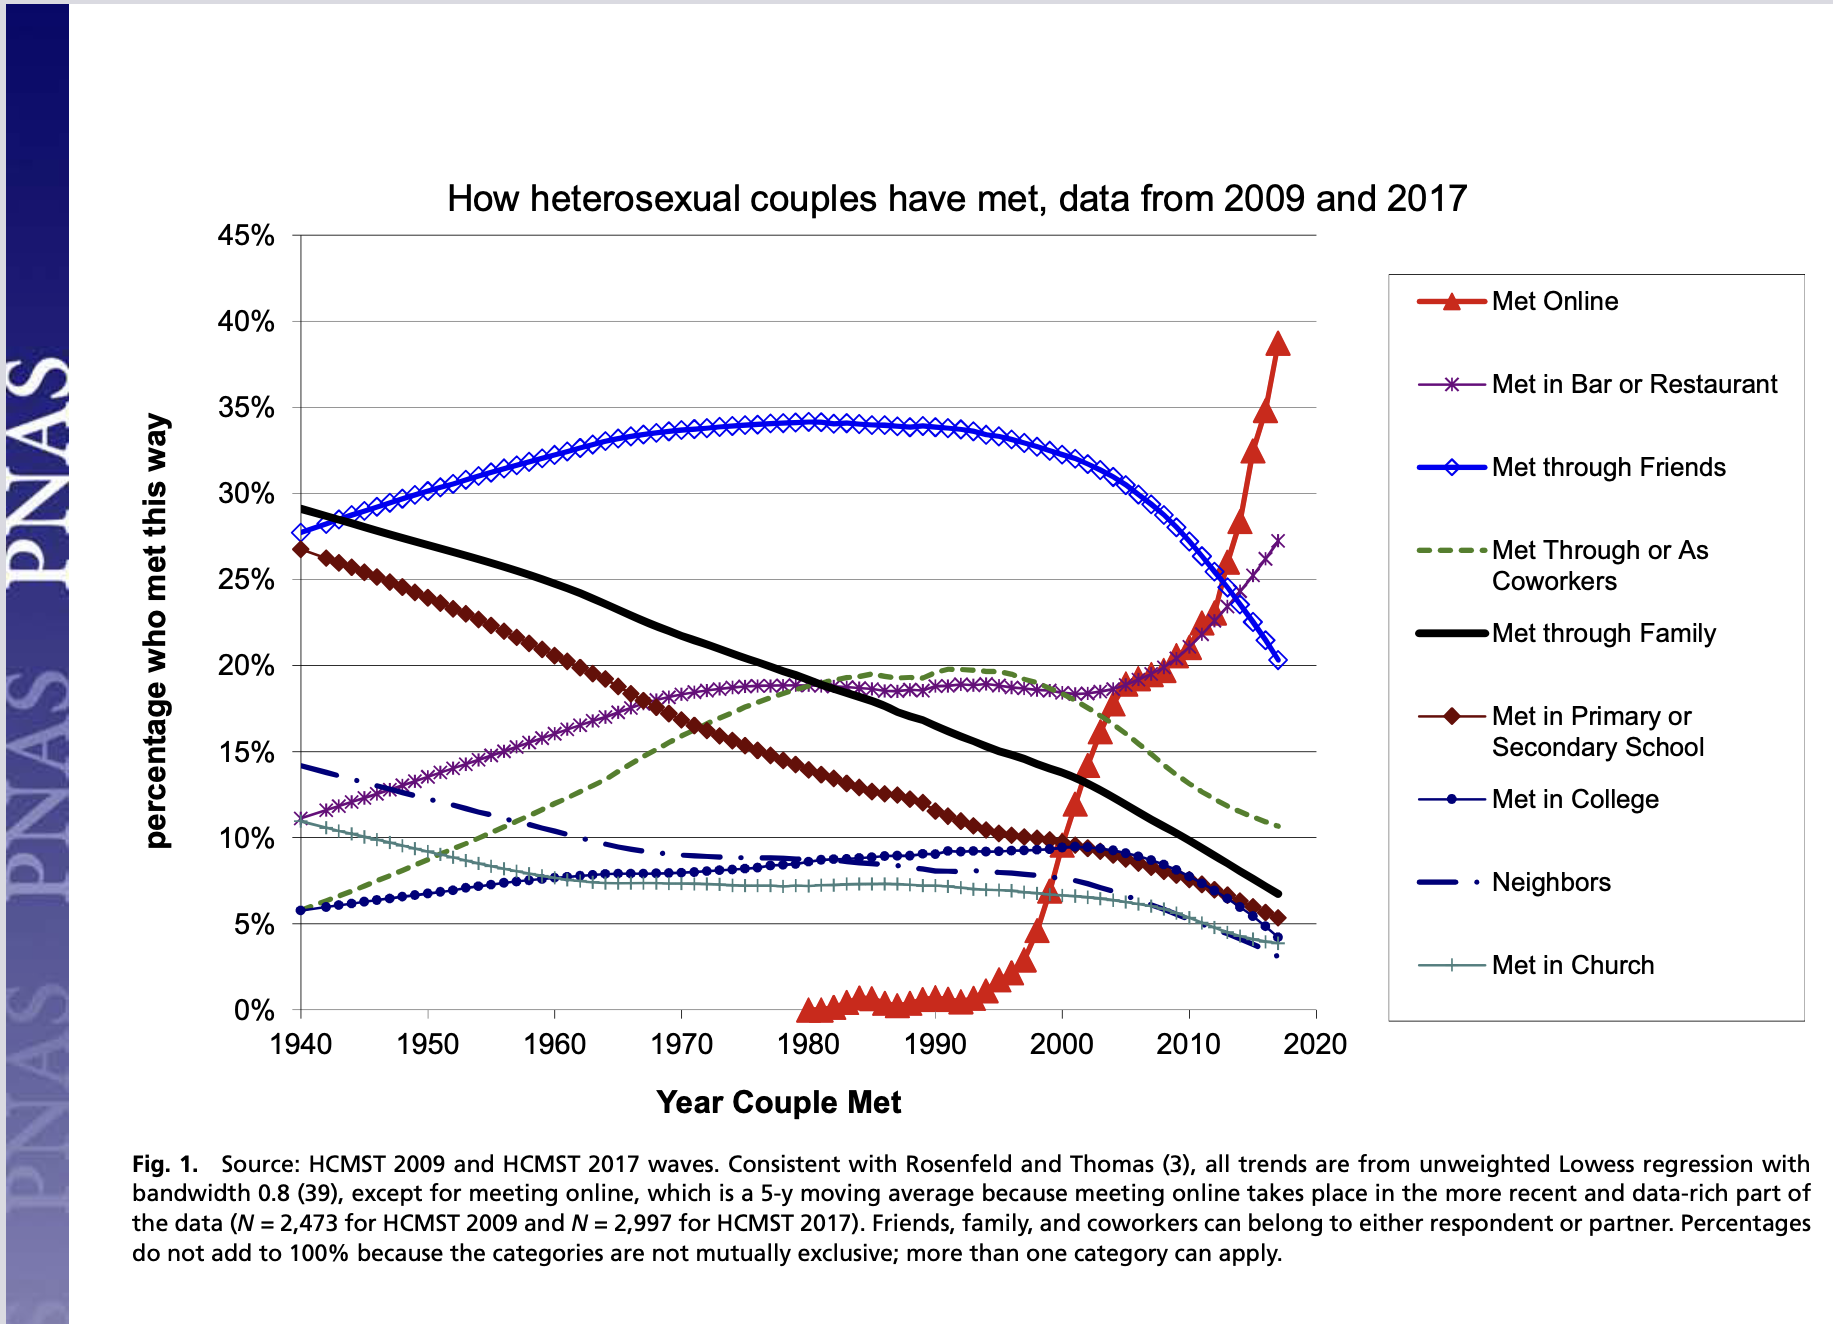
\includegraphics[width=\linewidth,height=0.84\textheight,keepaspectratio]{figures/online_dating.png}
\end{center}
\end{frame}

%% ---------- CONCEPTUAL FRAMEWORK (after How heterosexual couples meet) ----------
\begin{frame}[shrink=5]{Conceptual framework}
\vspace{0.3em}
\begin{itemize}\small\setlength\itemsep{0.45em}
  \item Online dating is thought to \highlight{reduce search frictions} and thicken romance markets.
  \begin{itemize}\small\setlength\itemsep{0.3em}
    \item It could create long-term partnerships where families are an intentional choice.
    \item It could therefore \highlight{increase} birth rates for the marginal couple.
  \end{itemize}
  \item But complaints have risen that online dating causes \highlight{``permanent dating,''} which could reduce births.
  \begin{itemize}\small\setlength\itemsep{0.3em}
    \item These are profit-maximizing, publicly traded firms with arguably concentrated ownership, an \highlight{HHI around 4{,}500} (Match owns $\sim$75 of the platforms).
    \item They may, purposefully or inadvertently, design interfaces to \highlight{minimize exit} from the market through romantic matches, exactly the ``permanent dating'' channel.
  \end{itemize}
\end{itemize}
\vspace{0.3em}
\emphbox{This is an old version of the study, but a real dataset with a real treatment assignment (not simulated). It is presented as a vehicle for thinking about staggered adoption, CS, and how diagnostics uncovered problems.}
\end{frame}

%% ============================================================
%% CHECKLIST STEP 1 — DEFINE THE TARGET PARAMETER
%% ============================================================

\begin{frame}{Checklist step 1: define the target parameter}
\vspace{0.5em}
Recall that all average treatment effects have \highlight{three ingredients}:
\vspace{0.4em}
\begin{enumerate}\setlength\itemsep{0.6em}
  \item Potential outcomes representing treatment effects.
  \item Populations of units at a point in time.
  \item Weighted expectations.
\end{enumerate}
\vspace{0.6em}
\emphbox{So we have to make a \textbf{design} decision: which treatment effect will we target, and why?}
\end{frame}

\begin{frame}[shrink=5]{Checklist step 1: define the target parameter}
\vspace{0.2em}
\begin{center}\large Treatment effect: $\;\delta_i = Y_i(1) - Y_i(0)$\end{center}
\vspace{0.4em}
\begin{itemize}\small\setlength\itemsep{0.45em}
  \item I start with a binary indicator and will explain momentarily which intervention I use.
  \item Don't think in terms of ``the treatment effect,'' because there is no single ``the.''
  \item Imagine you had trillions of euros and permission to run any randomized trial you wanted.
  \item You would randomize \highlight{two} things, not one: $Y(1)$ is ``received online dating.''
  \item But what is $Y(0)$?
  \item In a trial the comparison group isn't given ``no medicine,'' but a \highlight{different} treatment, usually a sugar pill.
\end{itemize}
\end{frame}

\begin{frame}{Checklist step 1: define the target parameter}
\vspace{0.5em}
\begin{itemize}\setlength\itemsep{0.8em}
  \item You have to decide up front: what state of the world is the most relevant comparison for you?
  \item Let's look at the history of online dating to motivate the \highlight{different} parameters we could estimate.
  \item Consider two eras: the early \highlight{open-website} period and the late \highlight{swiping} period.
\end{itemize}
\end{frame}

%% ---------- HISTORY OF ONLINE DATING (inside step 1) ----------
\begin{frame}{History of online dating}
\begin{center}
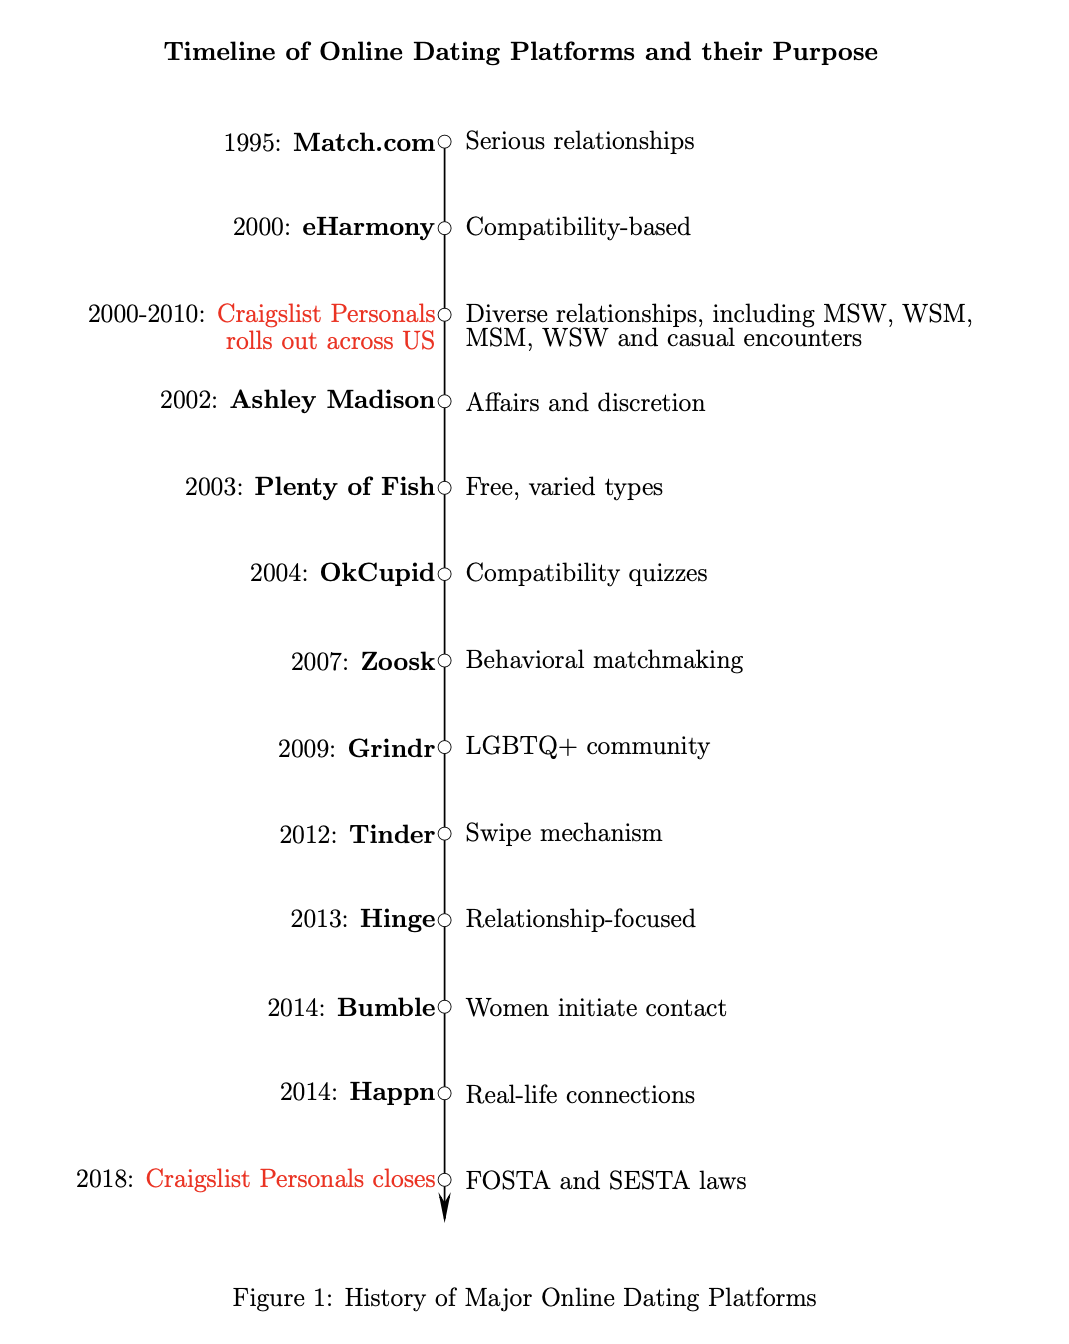
\includegraphics[width=\linewidth,height=0.82\textheight,keepaspectratio]{figures/onlinedating_timeline.png}
\end{center}
\end{frame}

\begin{frame}[shrink=5]{Checklist step 1: the open-website era}
\vspace{0.2em}
\begin{itemize}\small\setlength\itemsep{0.45em}
  \item In the 1990s and early 2000s, online dating was dominated by \highlight{Match, OKCupid, and eHarmony}.
  \item These were ``open websites'': anyone could use them, so selection into use was deeply endogenous without external variation.
  \item You would need an instrument (a LATE), matching on observables, or something more parametric.
  \item The upside is that the counterfactual is more plausibly $Y(0) =$ a world \highlight{without} online dating, simply because it is so early.
  \item But in this era online dating was mainly a path to life partners, not casual dating.
  \item It was also less common, and often \highlight{stigmatizing} as a signal of ``failure on the marriage market.''
\end{itemize}
\end{frame}

\begin{frame}[shrink=3]{Checklist step 1: the swiping era}
\vspace{0.2em}
\begin{itemize}\small\setlength\itemsep{0.5em}
  \item The later ``swiping'' era is different, and in many ways it is \highlight{the} contemporary platform people experience now.
  \item This is hard, because $Y(0)$ is probably \highlight{not} ``a world without online dating'': that world has stopped existing.
  \item Much more plausibly, $Y(0)$ means ``a \highlight{different} online dating platform.''
  \item This is also a period when online dating is much more common.
  \item After Tinder, this is the rise of \highlight{casual-sex} online dating.
\end{itemize}
\end{frame}

\begin{frame}{Checklist step 1: picking your treatment effect}
\vspace{0.5em}
\begin{center}\large
$\delta = Y(\text{online dating}) - Y(\text{friends and family})$\\[0.7em]
versus\\[0.7em]
$\delta = Y(\text{online dating platform 1}) - Y(\text{online dating platform 2})$
\end{center}
\vspace{0.6em}
\begin{itemize}\small\setlength\itemsep{0.45em}
  \item You have to decide which of these you care about, and make your design decisions around it.
  \item I target the \highlight{first}, with $Y(\text{friends and family}) = 0$ as my counterfactual, which means going further back in time.
  \item I also go back because the post-2008 period is rife with \highlight{confounders}.
\end{itemize}
\end{frame}

%% ---------- NATIONAL BIRTH RATE ----------
\begin{frame}{The national birth rate}
\begin{center}
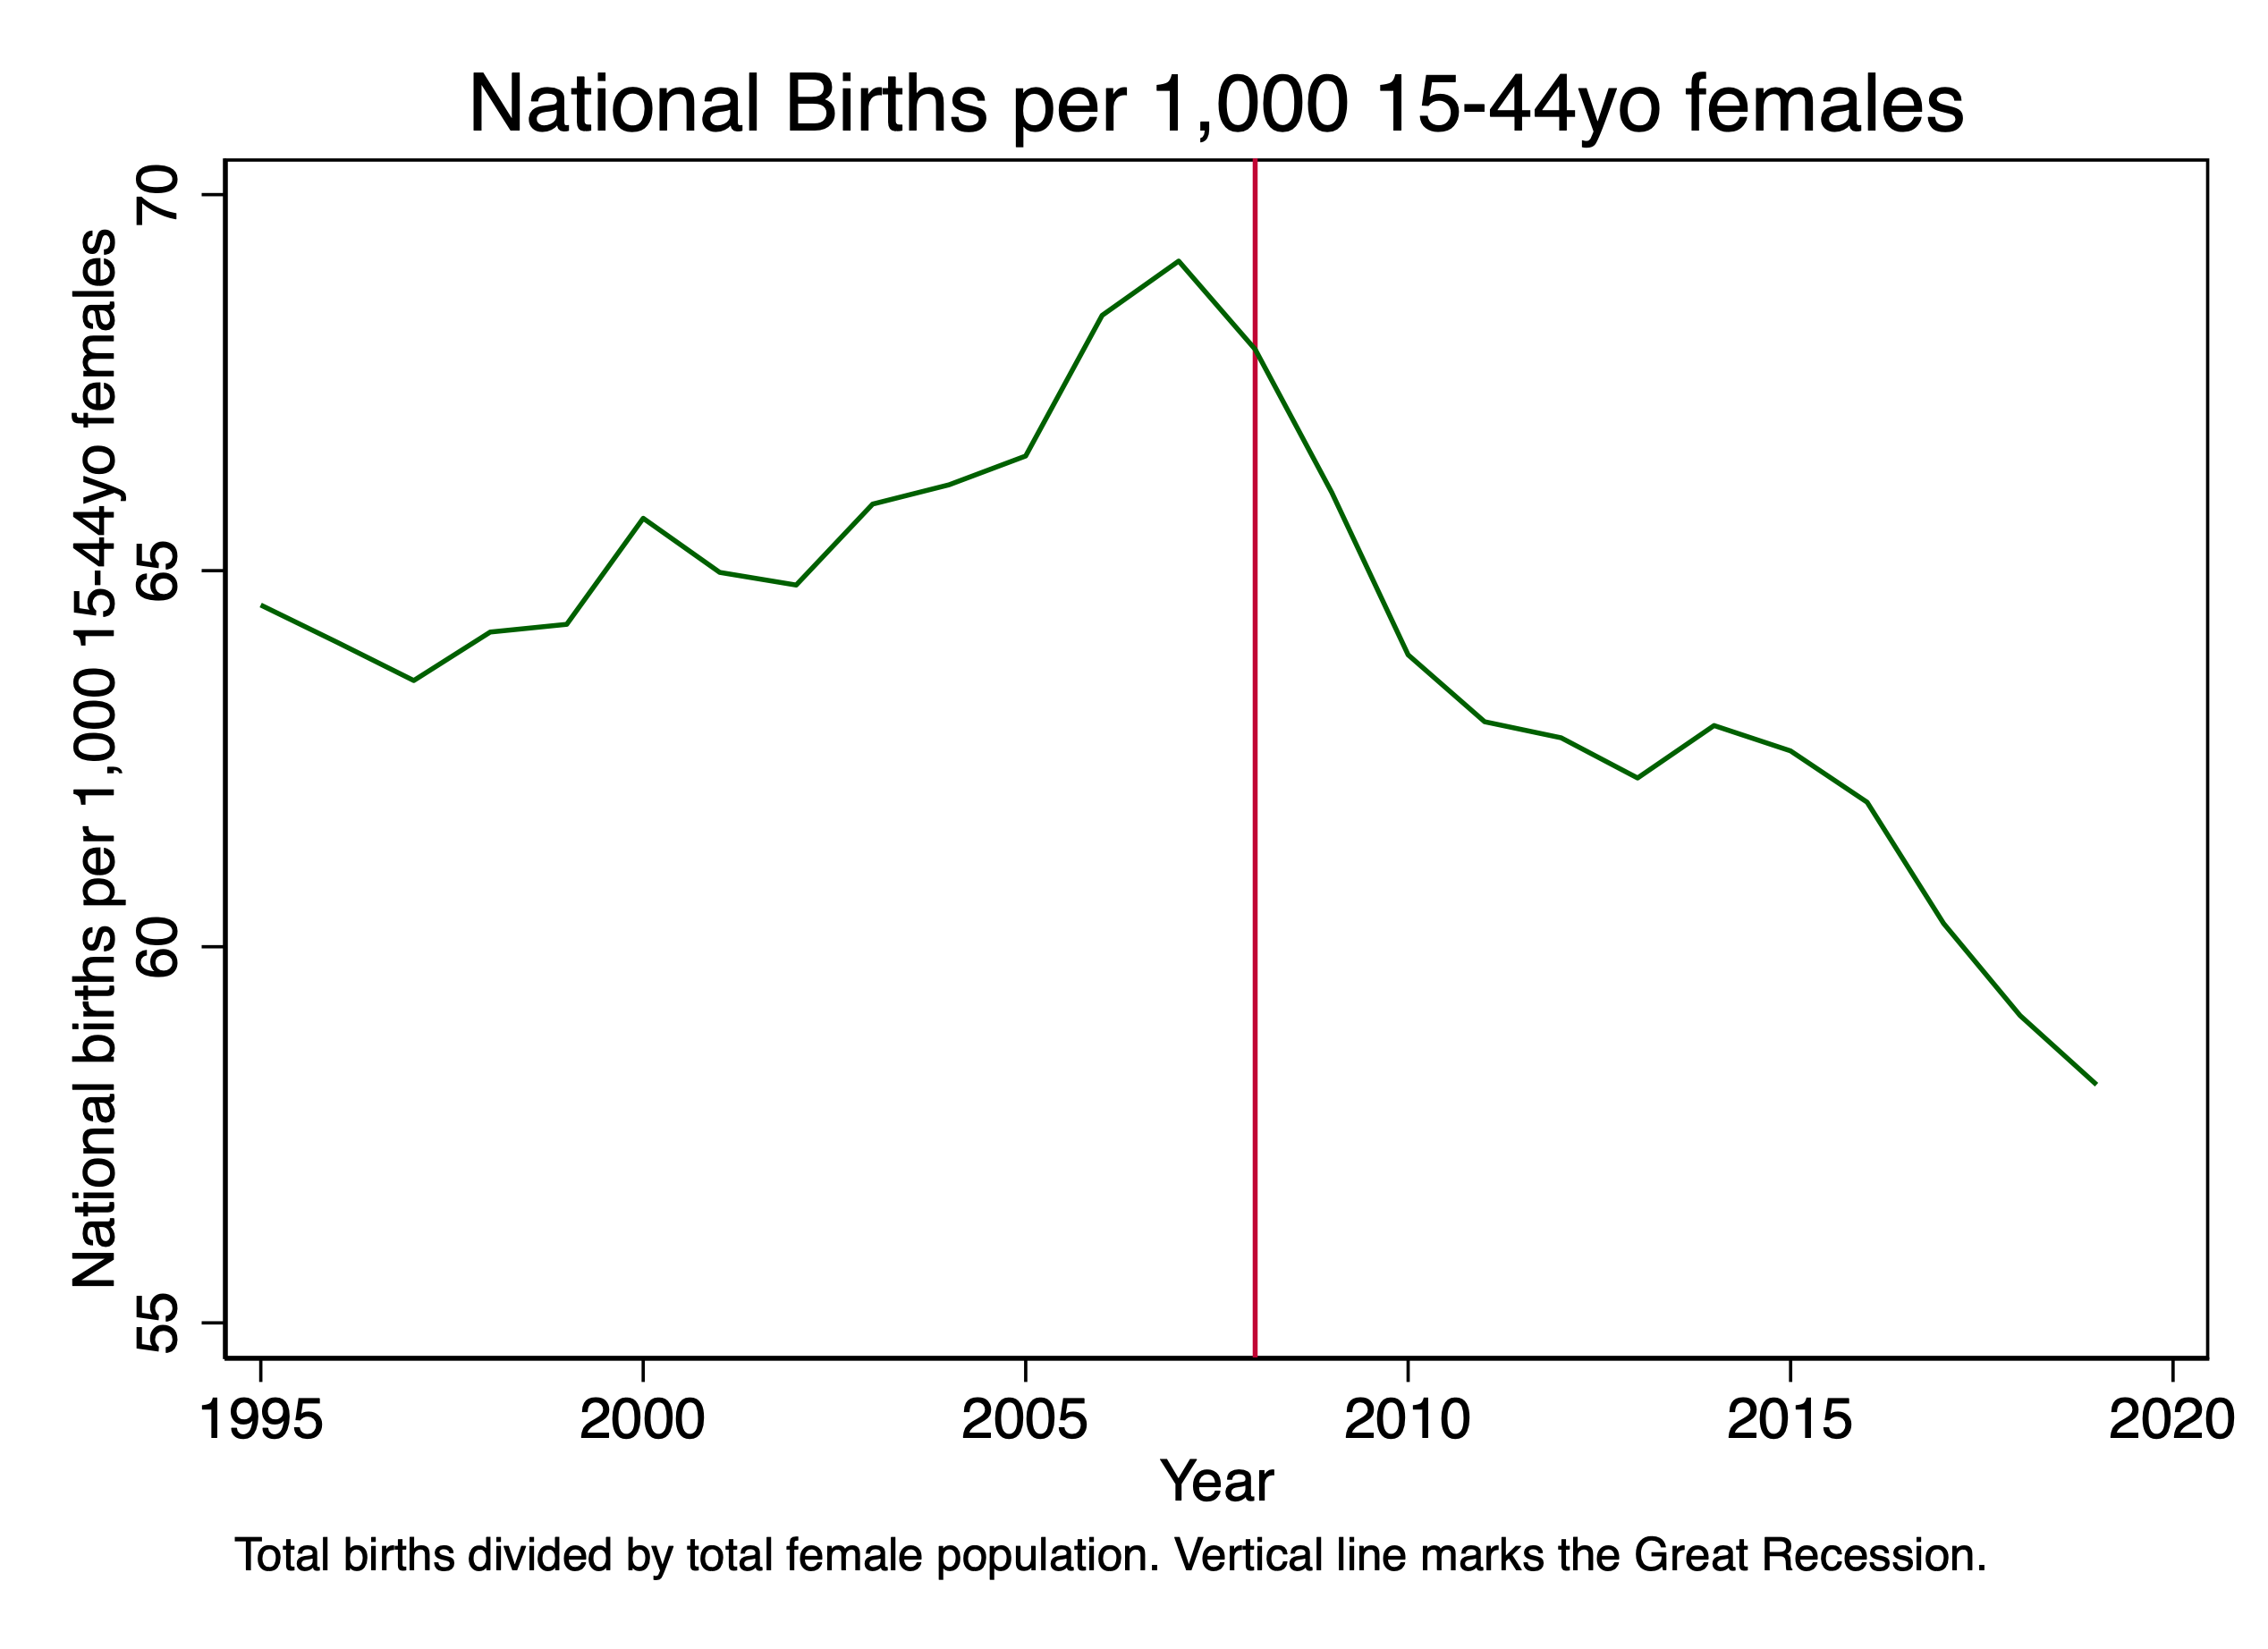
\includegraphics[width=\linewidth,height=0.84\textheight,keepaspectratio]{figures/national_br.png}
\end{center}
\end{frame}

%% ---------- GSS LONG-ARC (before Confounders) ----------
\begin{frame}{The dating market has changed structurally since 1972}
\begin{center}
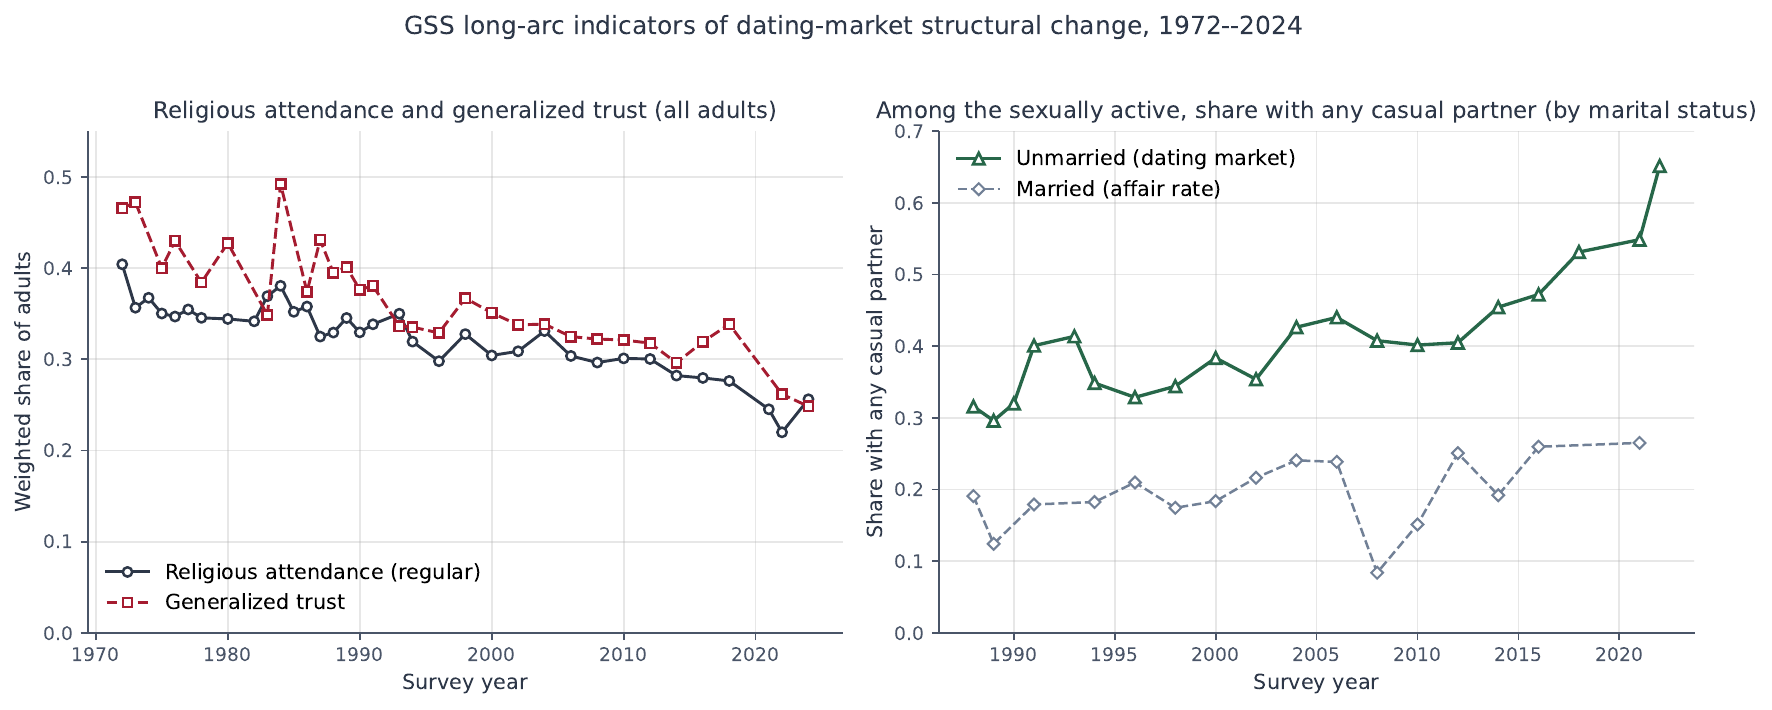
\includegraphics[width=\linewidth,height=0.84\textheight,keepaspectratio]{figures/str_gss_long_run.png}
\end{center}
\end{frame}

%% ---------- CONFOUNDERS ----------
\begin{frame}{Confounders}
\vspace{0.3em}
\textbf{Two problems:}
\begin{enumerate}\small\setlength\itemsep{0.4em}
  \item Online dating either hits the US with an \highlight{open website} anyone can get on (early period) or a \highlight{``swiping app''} anyone can get on (late period).
  \item After 2008, American birth rates \highlight{plummeted and never recovered} (demographic transition).
\end{enumerate}
\vspace{0.5em}
\begin{itemize}\small\setlength\itemsep{0.4em}
  \item Both are massive, hurricane-like winds, and it's going to be challenging to deal with them with diff-in-diff.
  \item But, amazingly, we have a solution that gets at \emph{both} and is probably much closer to our target parameter, \highlight{Craigslist Personals}.
\end{itemize}
\end{frame}

%% ---------- BIRTH RATES DIGITAL TIMELINE (after Confounders) ----------
\begin{frame}{Birth rates and the digital dating timeline}
\begin{center}
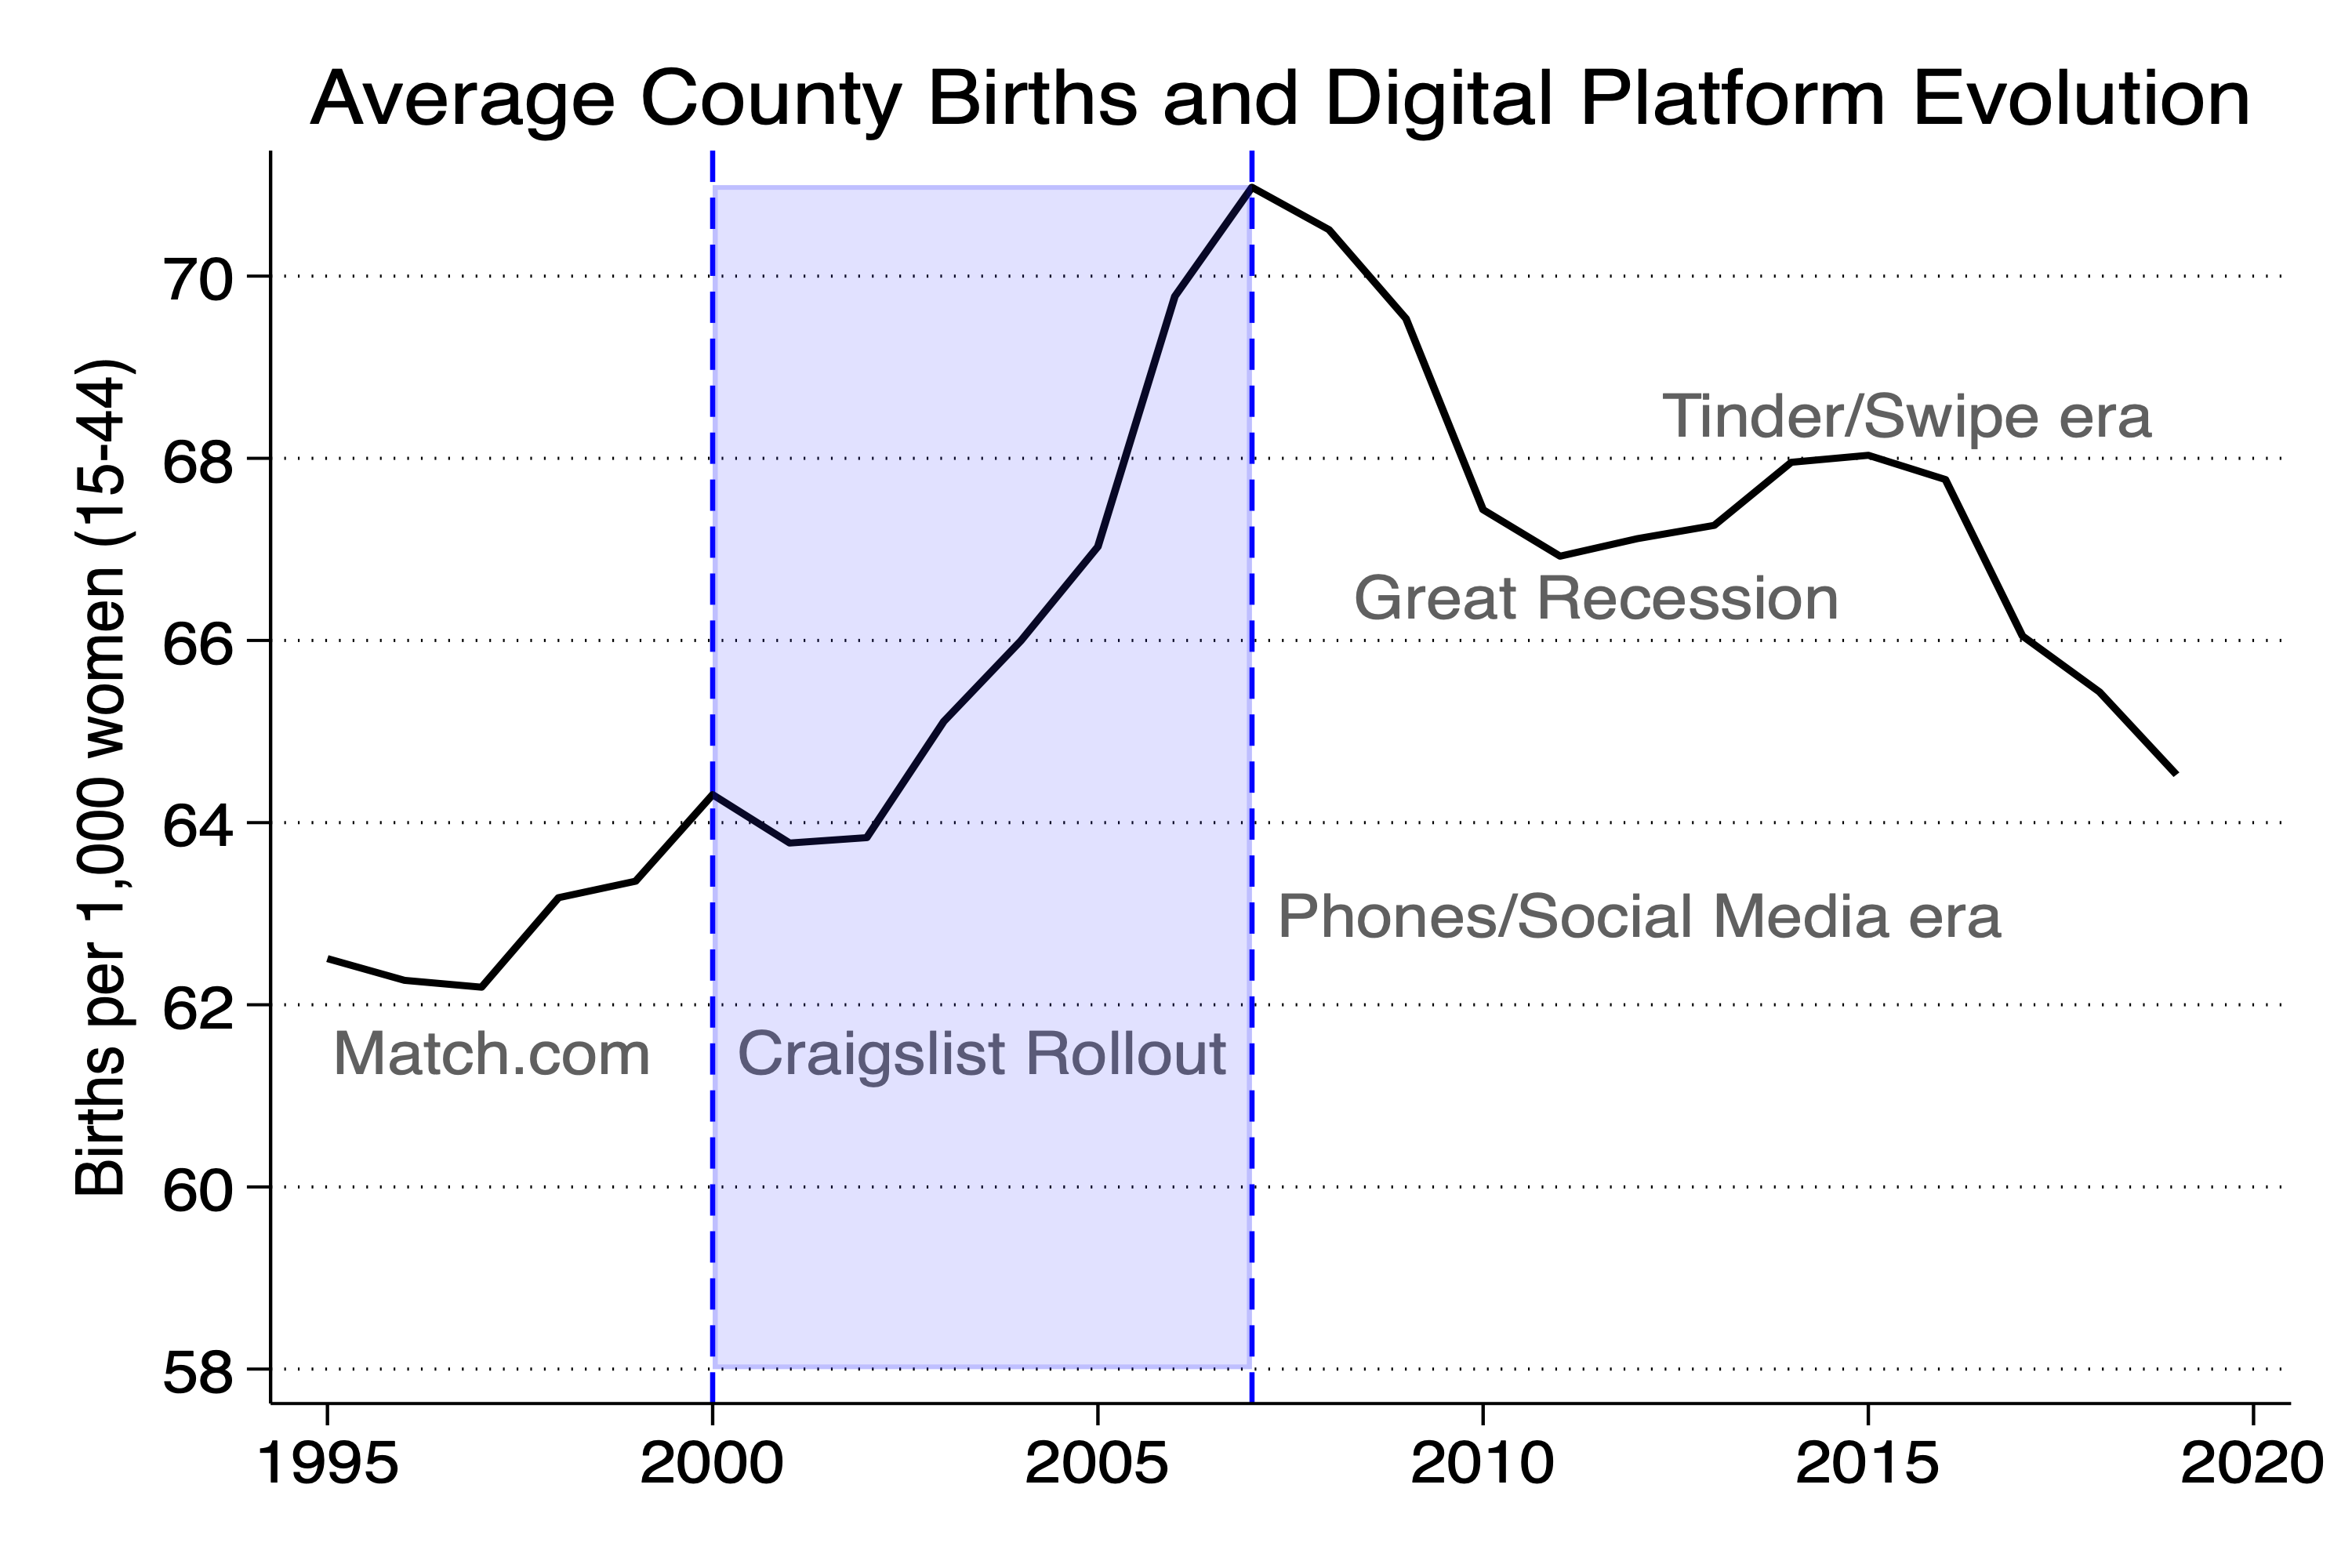
\includegraphics[width=\linewidth,height=0.84\textheight,keepaspectratio]{figures/birth_rates_digital_timeline.png}
\end{center}
\end{frame}

%% ---------- DATA SELECTION ----------
\begin{frame}{Data selection}
\vspace{0.3em}
\begin{itemize}\small\setlength\itemsep{0.4em}
  \item We focused originally on \highlight{birth rates for 15--44yo females}; the unit of observation is the \highlight{county}.
  \item Sample period: \highlight{1995} (when Craigslist first opens) to \highlight{2007}. Why 2007? Three reasons:
  \begin{enumerate}\small\setlength\itemsep{0.15em}
    \item Birth rates plummeted following the Great Recession (demographic transition).
    \item Online dating apps like Tinder appear simultaneously, no geographic variation to exploit.
    \item We wanted to avoid the social-media environment.
  \end{enumerate}
  \item We keep counties treated in 2008--2010 in the dataset as a sample of \highlight{``not-yet-treated''} counties.
  \item Used the \highlight{Wayback Machine} to find the exact month Craigslist Personals appeared in each county, assigned it to adjacent counties too, then coded a county-year as treated if it was ever treated.
\end{itemize}
\end{frame}

%% ---------- STEP 1: AVERAGING / WEIGHTING (follows Data selection) ----------
%% ---------- WAYBACK MACHINE (after Data selection) ----------
\begin{frame}{The Wayback Machine}
\vspace{0.5em}
\begin{itemize}\setlength\itemsep{0.7em}
  \item In my JHR with Greg DeAngelo and John Tripp, we used the \highlight{Wayback Machine} to identify the start dates of Craigslist opening erotic services.
  \item Here we use it to identify the dates when \highlight{Craigslist Personals} showed up.
  \item We went through every US city to find the exact date it got Craigslist Personals.
  \item Personals potentially linked the old website era of romance-oriented online dating with the modern swipe era and its stronger \highlight{casual-matching} component.
\end{itemize}
\vspace{0.4em}
\meta{Let's look at the history of Craigslist Personals.}
\end{frame}

%% ---------- HISTORY OF CRAIGSLIST PERSONALS (melanie2--8) ----------
\begin{frame}{The history of Craigslist Personals}
\begin{center}
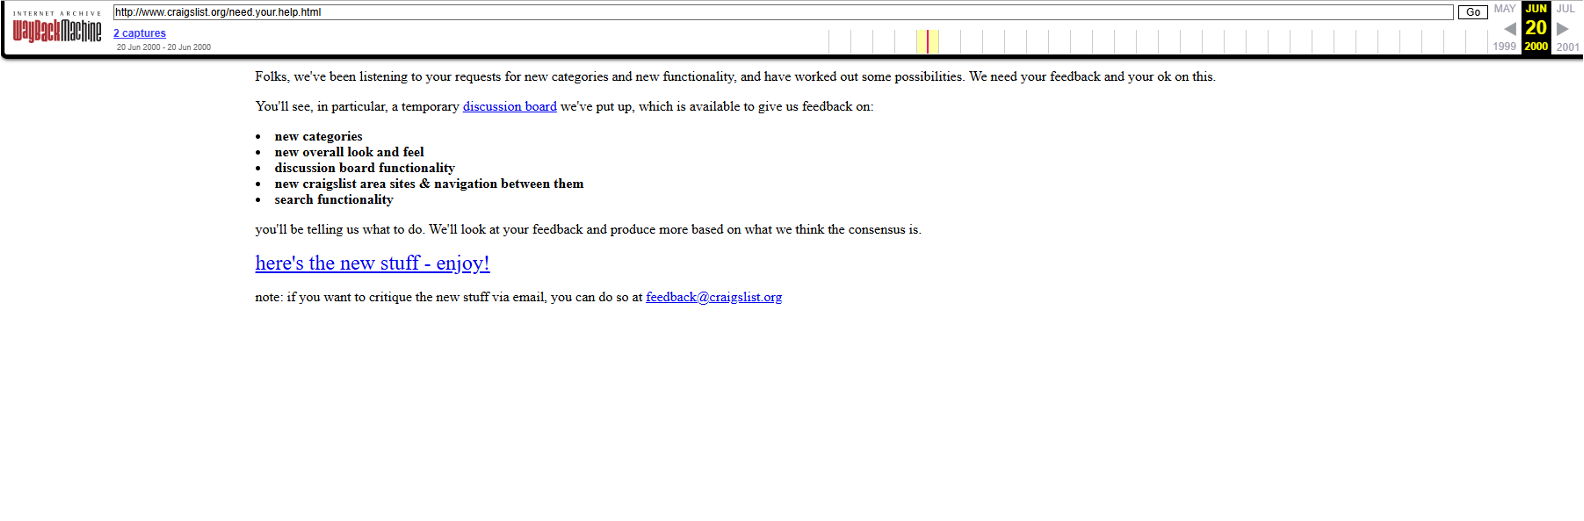
\includegraphics[width=\linewidth,height=0.80\textheight,keepaspectratio]{figures/melanie2.png}
\end{center}
\end{frame}

\begin{frame}{The history of Craigslist Personals}
\begin{center}
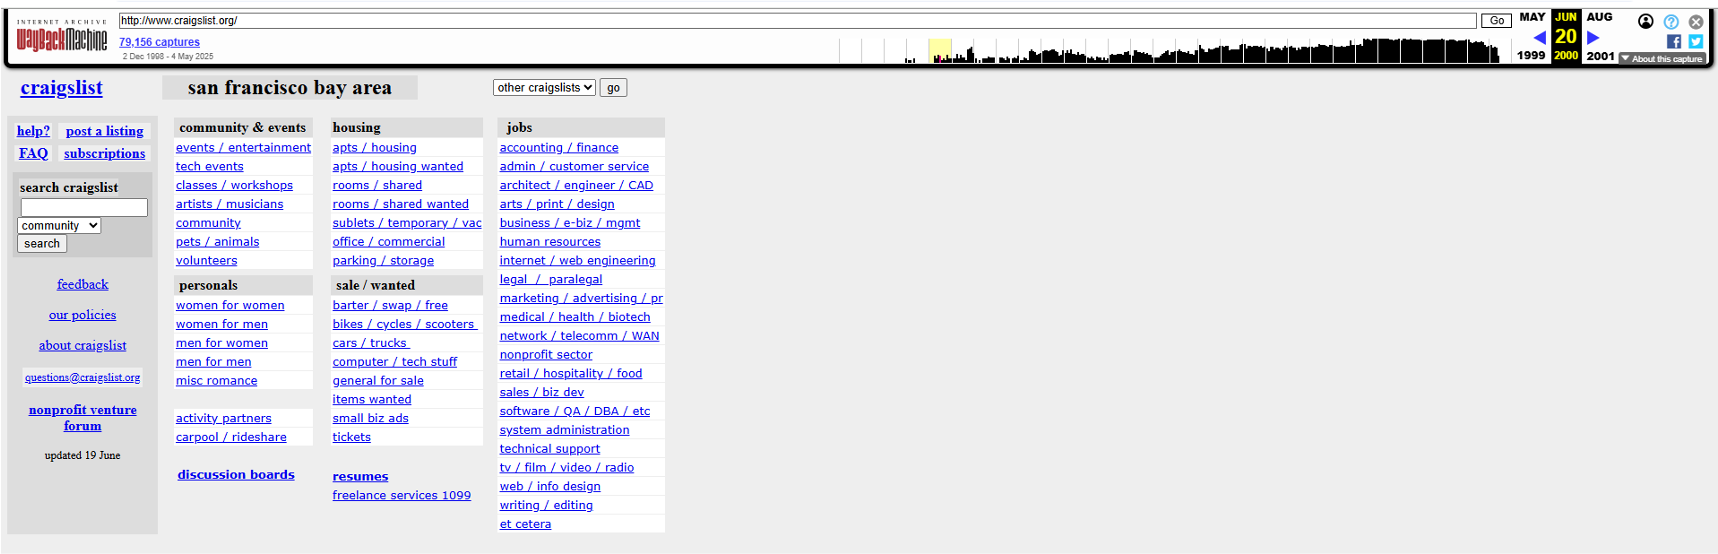
\includegraphics[width=\linewidth,height=0.80\textheight,keepaspectratio]{figures/melanie3.png}
\end{center}
\end{frame}

\begin{frame}{The history of Craigslist Personals}
\begin{center}
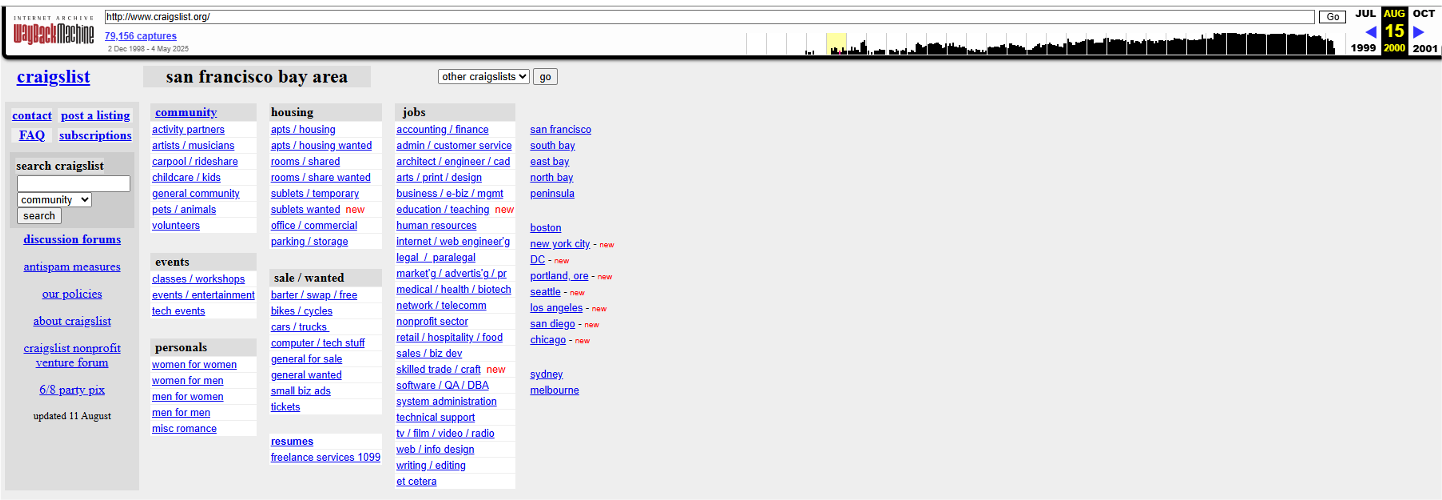
\includegraphics[width=\linewidth,height=0.80\textheight,keepaspectratio]{figures/melanie4.png}
\end{center}
\end{frame}

\begin{frame}{The history of Craigslist Personals}
\begin{center}
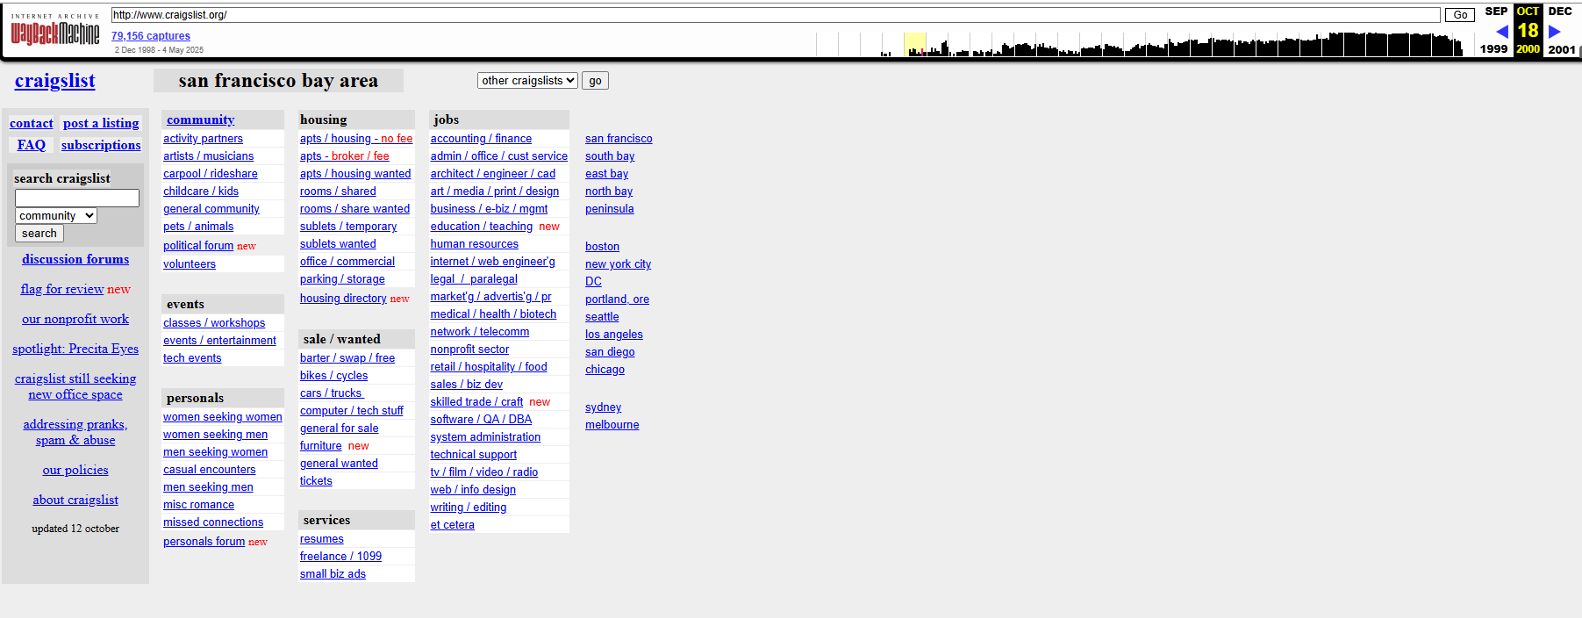
\includegraphics[width=\linewidth,height=0.80\textheight,keepaspectratio]{figures/melanie5.png}
\end{center}
\end{frame}

\begin{frame}{The history of Craigslist Personals}
\begin{center}
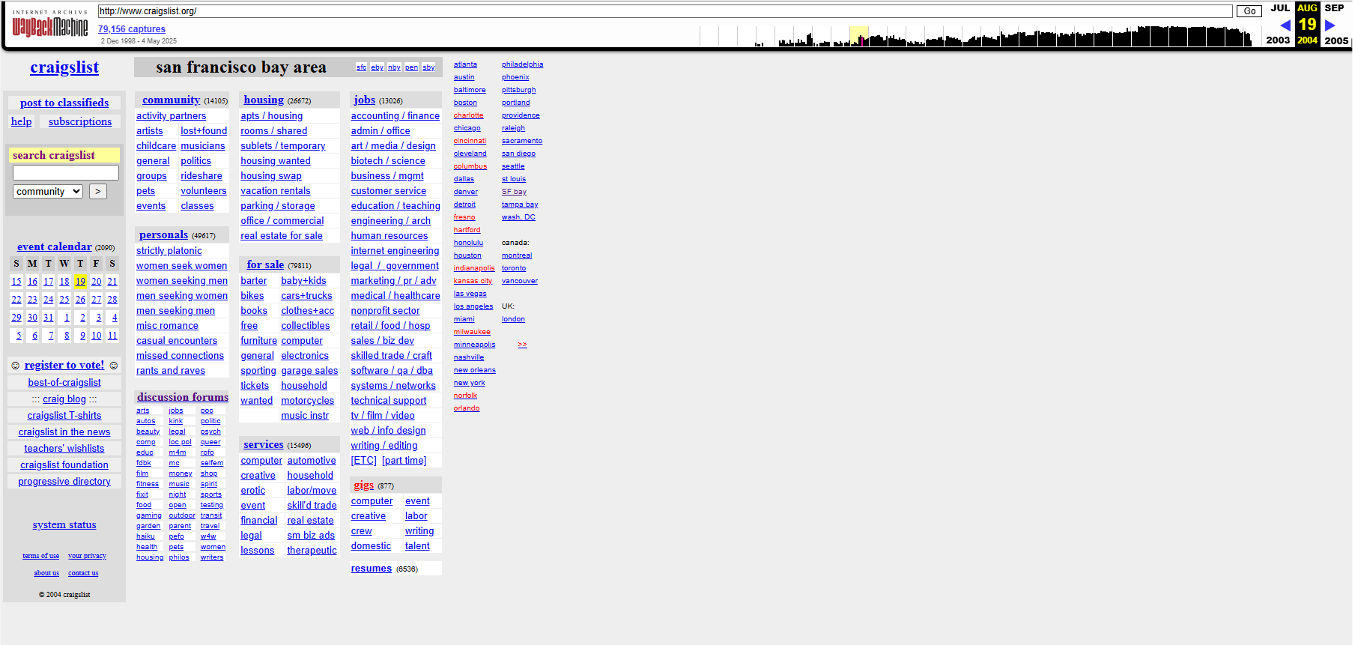
\includegraphics[width=\linewidth,height=0.80\textheight,keepaspectratio]{figures/melanie6.png}
\end{center}
\end{frame}

\begin{frame}{The history of Craigslist Personals}
\begin{center}
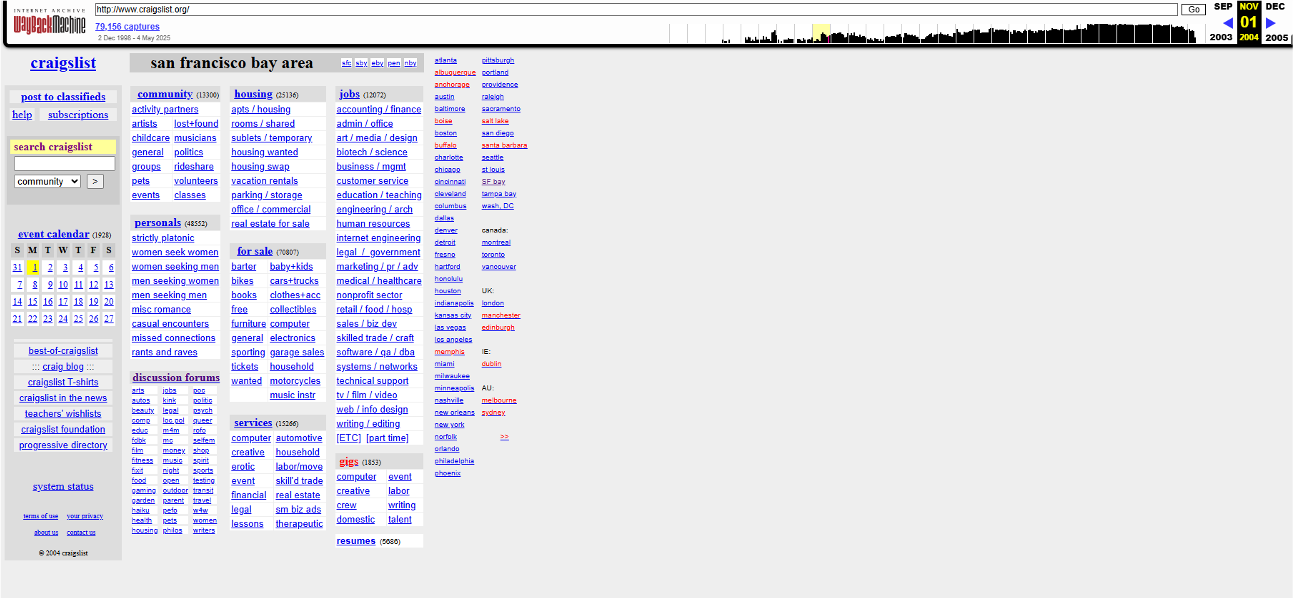
\includegraphics[width=\linewidth,height=0.80\textheight,keepaspectratio]{figures/melanie7.png}
\end{center}
\end{frame}

\begin{frame}{The history of Craigslist Personals}
\begin{center}
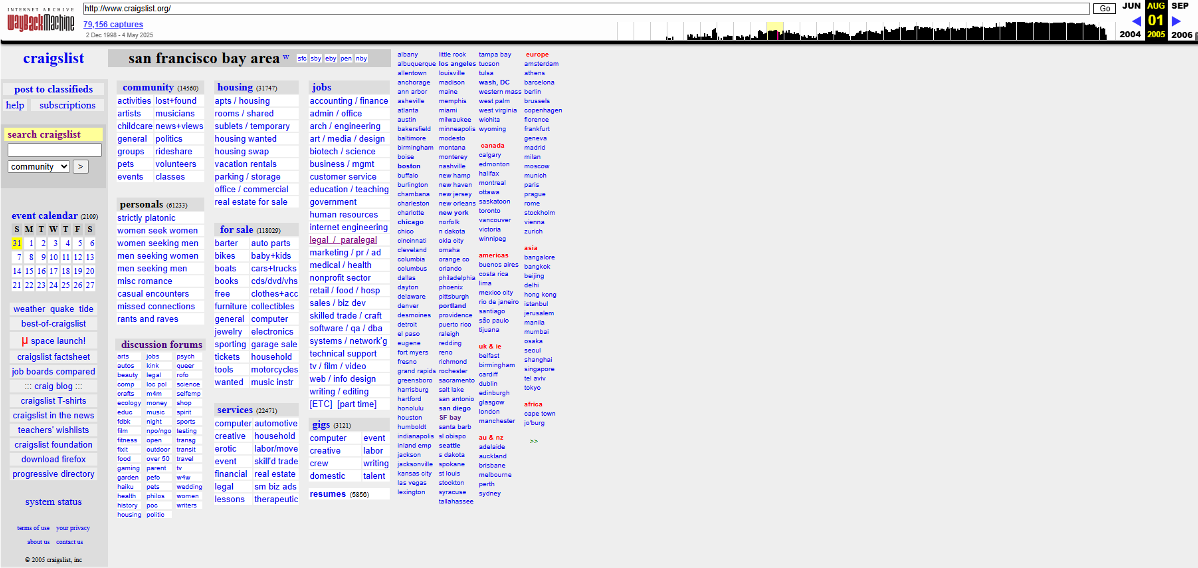
\includegraphics[width=\linewidth,height=0.80\textheight,keepaspectratio]{figures/melanie8.png}
\end{center}
\end{frame}

%% ---------- CRAIGSLIST ROLLOUT BY PHASES ----------
\begin{frame}{Craigslist rolled out in geographic phases}
\begin{center}
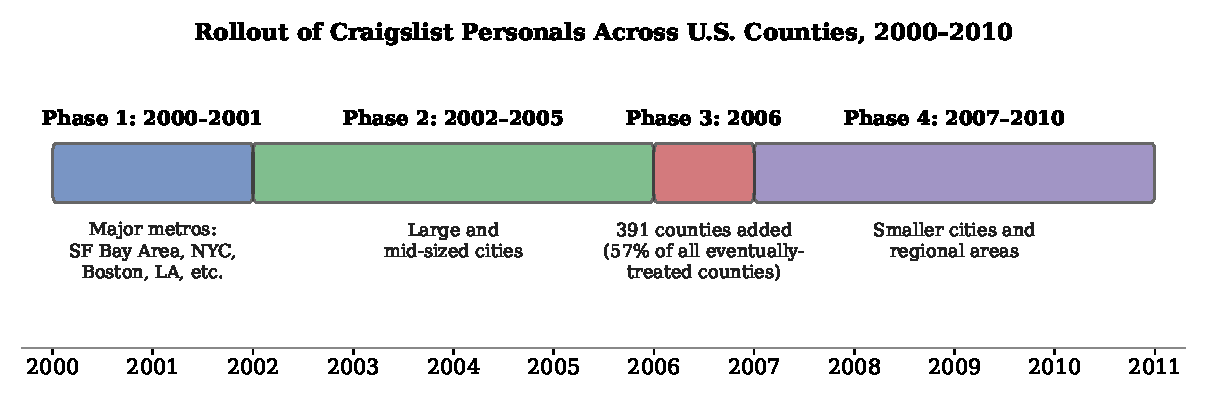
\includegraphics[width=\linewidth,height=0.84\textheight,keepaspectratio]{figures/CL_rollout_byPhases.pdf}
\end{center}
\end{frame}

%% ---------- CHECKLIST STEP 1: AVERAGING / WEIGHTING ----------
\begin{frame}[shrink=5]{Checklist step 1: what will our average causal effect be?}
\vspace{0.3em}
\begin{itemize}\small\setlength\itemsep{0.5em}
  \item We are focused on marriage markets, so we target the \highlight{unweighted} (or simply weighted) average of county-level treatment effects.
  \begin{itemize}\small\setlength\itemsep{0.35em}
    \item Without population weights, you average over the units of observation, here counties, so you estimate the effect for the \highlight{average county}.
    \item With population weights, large counties get larger and small counties get smaller, so you estimate the effect for the \highlight{average woman}.
    \item Both are interesting, but they differ, and need not line up or even share a sign under heterogeneous treatment effects.
  \end{itemize}
\end{itemize}
\end{frame}

\begin{frame}{Checklist step 1: sample window and counterfactual}
\vspace{0.5em}
\begin{itemize}\setlength\itemsep{0.8em}
  \item We stop the sample in \highlight{2007}, because after that we believe the question is probably not answerable.
  \item We also want $Y(0)$ to be as close as possible to ``a world without online dating, but still reasonably popular.''
  \item \highlight{Craigslist} is our solution, and it has the geographic rollout we just saw.
\end{itemize}
\end{frame}

%% ---------- CHECKLIST STEP 2: MAKE A TABLE OF TREATED UNITS ----------
\begin{frame}[shrink=5]{Checklist step 2: make a table of treated units}
\vspace{0.3em}
\begin{itemize}\small\setlength\itemsep{0.5em}
  \item First we simply count by cohort.
  \item With staggered adoption, we need to know how many units are treated and how many are not, because we will have to make decisions later.
  \item Here is what we initially found, and note it has changed since: a set of counties were treated from 2000 to 2010.
  \item We don't want to use 2008--2010, because of the huge demographic transition, too many confounders for credible diff-in-diff, and our target-parameter choice.
  \item So we use the 2008--2010 counties as our primary comparison group, calling them the \highlight{``eventually treated.''}
\end{itemize}
\end{frame}

%% ---------- COUNTS AND SHARES BY COHORT (screenshot) ----------
\begin{frame}{Counts and shares by cohort}
\begin{center}
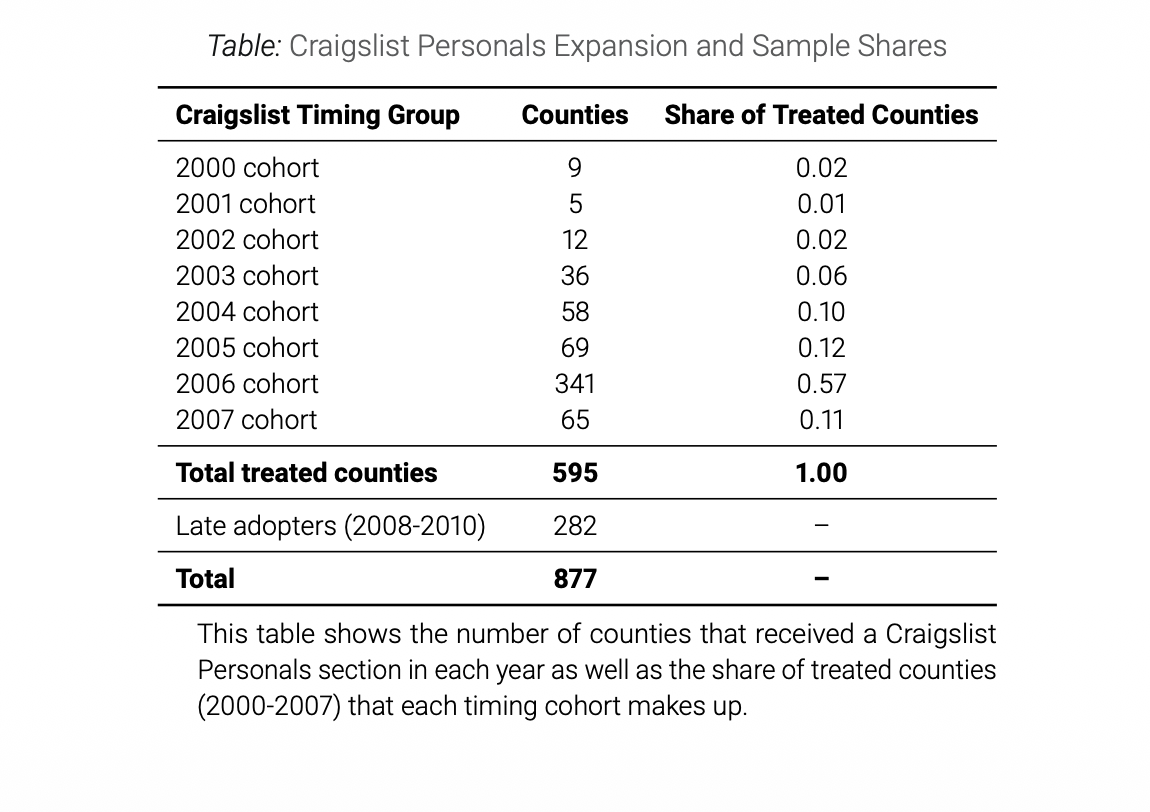
\includegraphics[width=\linewidth,height=0.82\textheight,keepaspectratio]{figures/counts_by_cohort.png}
\end{center}
\end{frame}

%% ---------- WHY GROUP SHARES AND COUNTS ----------
\begin{frame}[shrink=8]{Why group shares and counts}
\vspace{0.3em}
\begin{itemize}\small\setlength\itemsep{0.5em}
  \item Why we report cohort shares is a subtle point that is not well known.
  \item Whenever you average treatment effects across cohorts, you take a \emph{weighted} average based on \highlight{cohort size}.
  \item In an event study, the year-of-treatment ($t=0$) effect averages over \highlight{everyone}, since every cohort has a $t=0$.
  \item The 2006 cohort was a huge \highlight{57\%} of the treated group, so any aggregation including them is heavily swayed by them.
  \item But the $t=2$ effect drops the 2006 cohort, because the sample ends in 2007 and they have no $t+2$ in the data.
  \item Knowing the group shares tells you that any aggregation is a weighted average using those shares.
\end{itemize}
\end{frame}

%% ---------- STEP 3: PLOT TREATMENT ROLLOUT ----------
\begin{frame}{Checklist step 3: plot the treatment rollout}
\vspace{0.5em}
\begin{itemize}\setlength\itemsep{0.6em}
  \item Now create a visualization of the table we just made, plotting the rollout.
  \item I recommend \texttt{PanelView} by Yiqing Xu.
  \item It plots what you're looking for, and it also flags ``missing'' cells, so if counties suddenly vanish it reveals it.
  \item This helps you identify subtle issues ahead of time that are not easily found.
  \item Remember: you should have $N \times T$ units, with no surprises.
\end{itemize}
\end{frame}

\begin{frame}[plain]
\begin{center}
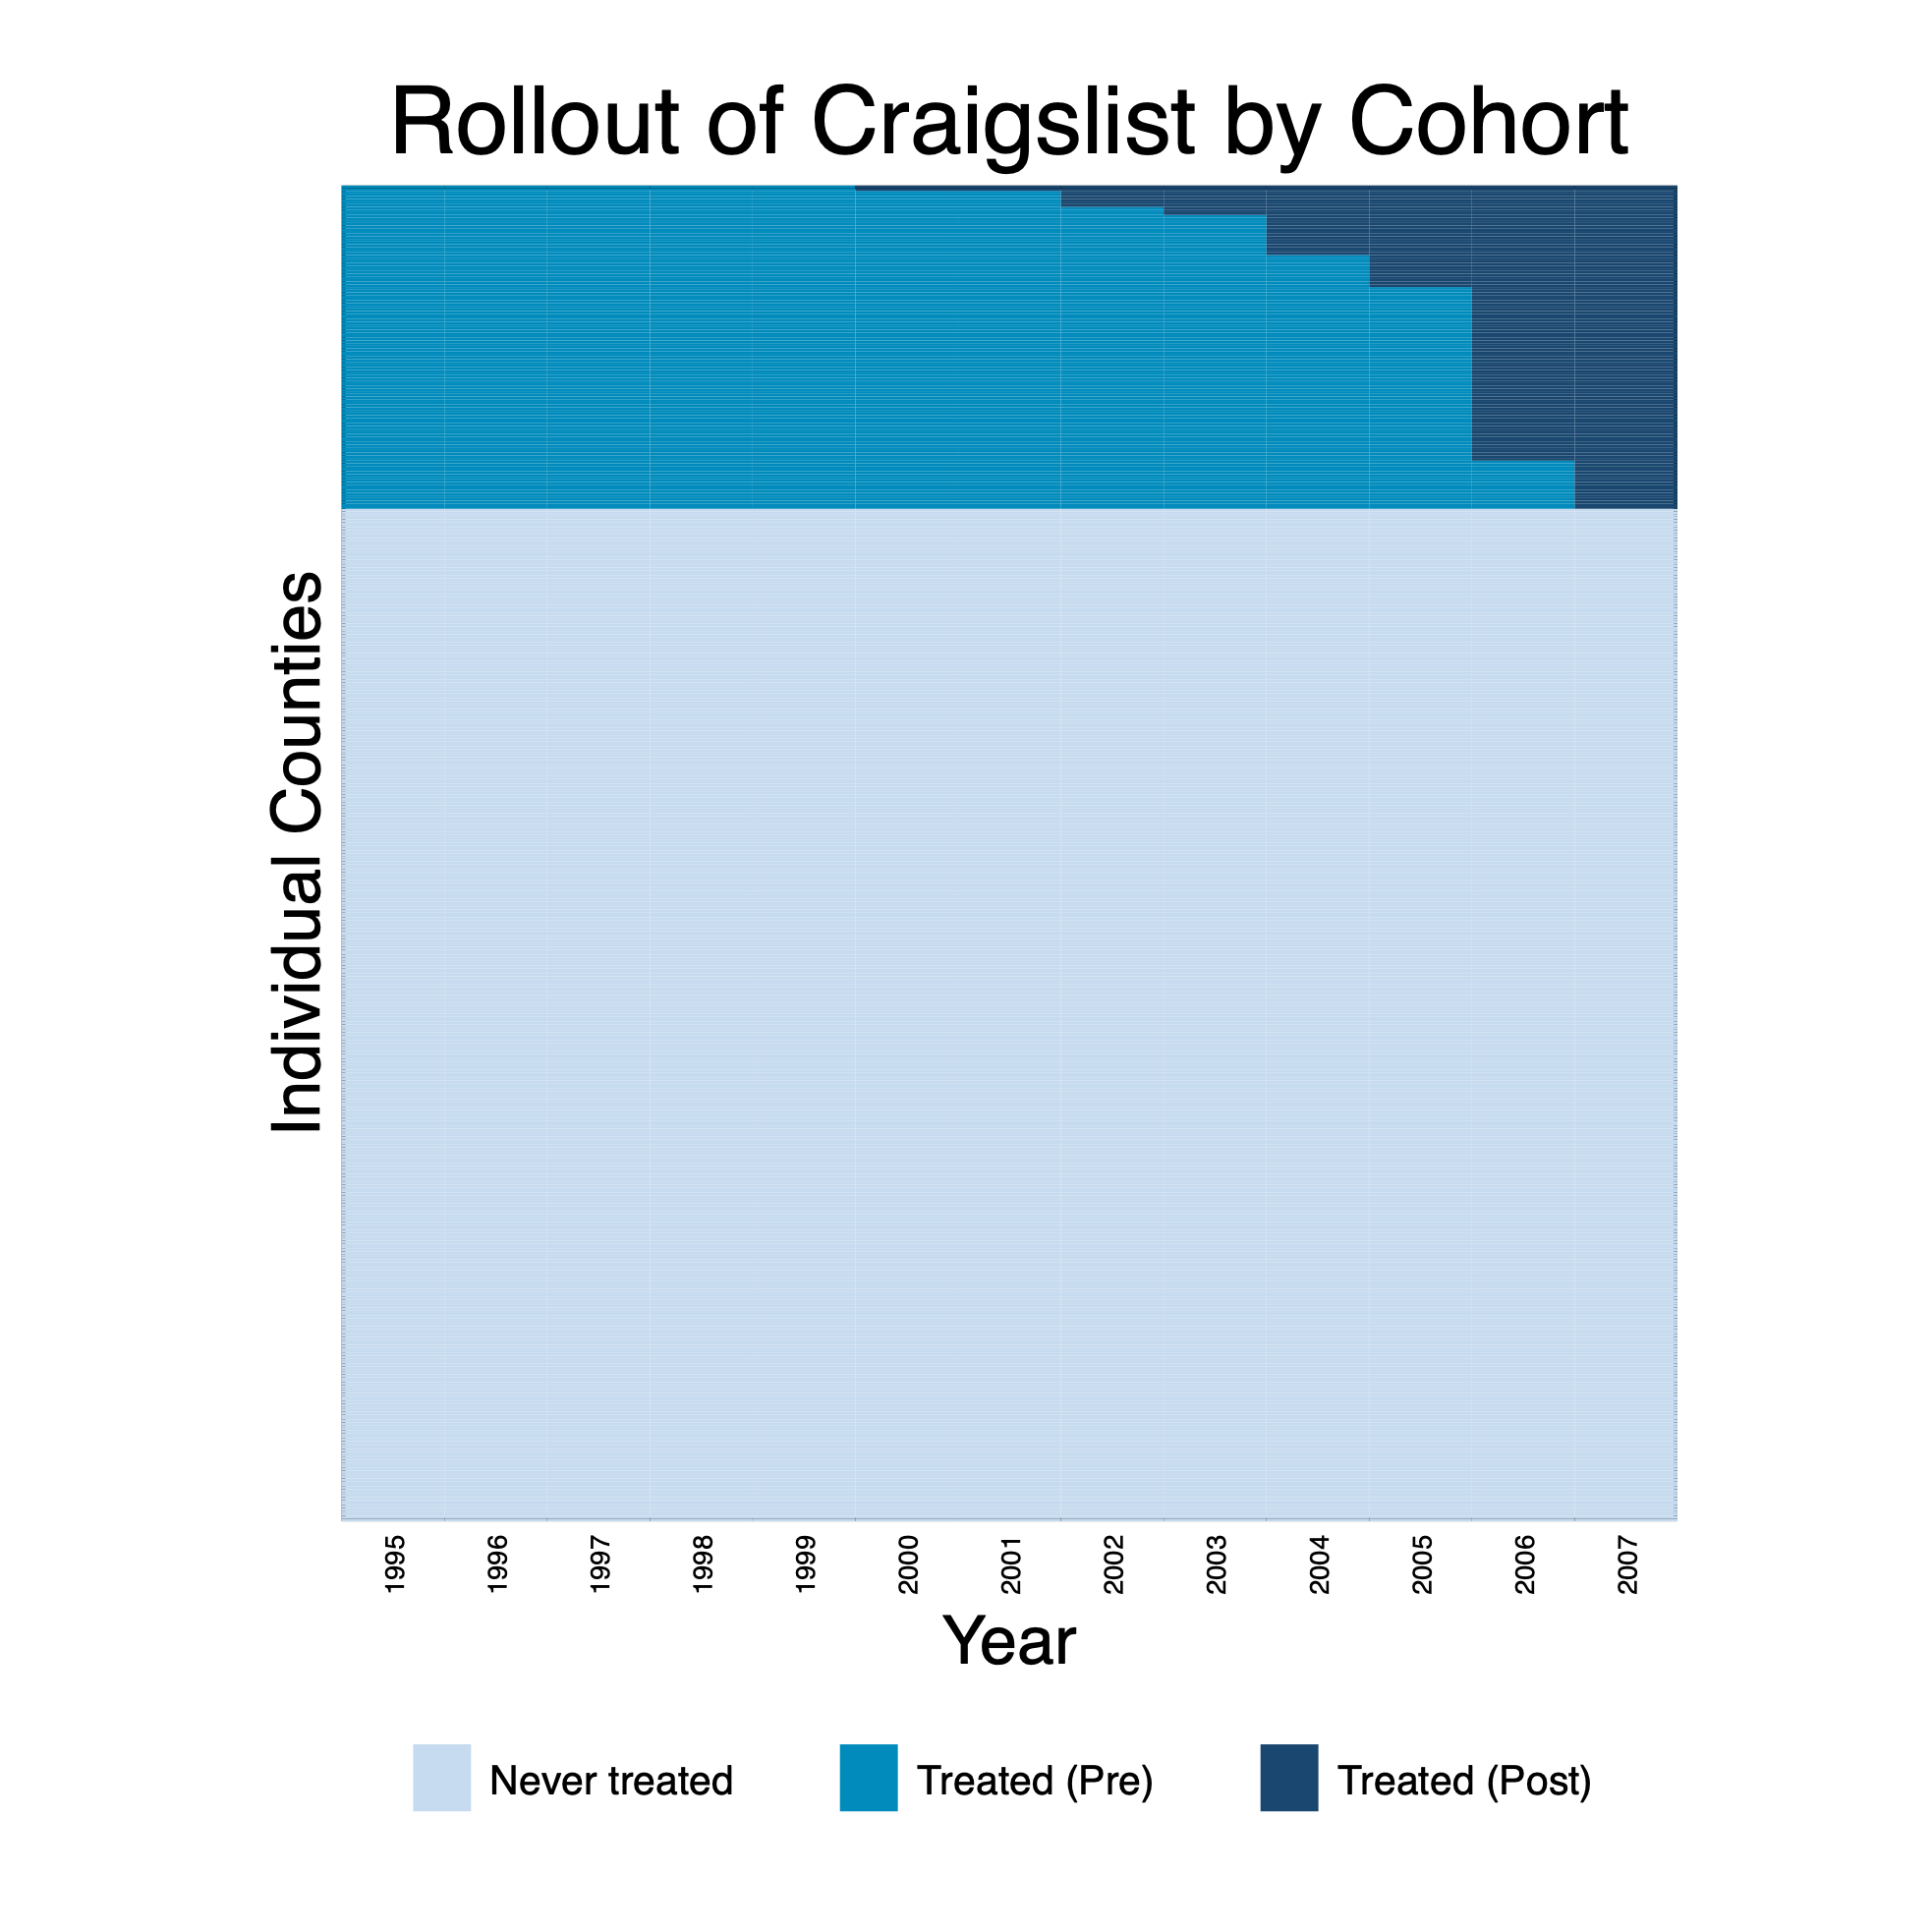
\includegraphics[width=0.98\paperwidth,height=0.94\paperheight,keepaspectratio]{figures/rollout.png}
\end{center}
\end{frame}

%% ---------- STEP 4: PICK YOUR COMPARISON GROUP ----------
\begin{frame}[shrink=5]{Checklist step 4: pick your comparison group}
\vspace{0.3em}
\begin{itemize}\small\setlength\itemsep{0.5em}
  \item You are usually choosing between the not-yet-treated, the never-treated, and the future-treated.
  \item Goodman-Bacon (2021) showed that the OLS twoway fixed effects estimator decomposes into a variance-weighted average of every 2$\times$2 in the data, including ones that use the \highlight{already-treated} as controls.
  \item You avoid those by manually computing 2$\times$2s per cohort with a robust DiD estimator, and we focus on \highlight{CS}.
  \item But you still have to decide who your control group is, and the \emph{only} criterion is: who do I believe parallel trends will hold for?
\end{itemize}
\end{frame}

\begin{frame}{Checklist step 4: pick your comparison group}
\vspace{0.5em}
\begin{itemize}\setlength\itemsep{0.7em}
  \item The never-treated and not-yet-treated are more interchangeable the more quasi-random assignment was, since then unobserved selection isn't driving assignment.
  \item Insofar as you are unsure, I think the \highlight{not-yet-treated} is probably better.
  \item So I actually wrote \highlight{Craig Newmark}, who started Craigslist, and asked him.
\end{itemize}
\end{frame}

\begin{frame}[plain]
\begin{center}
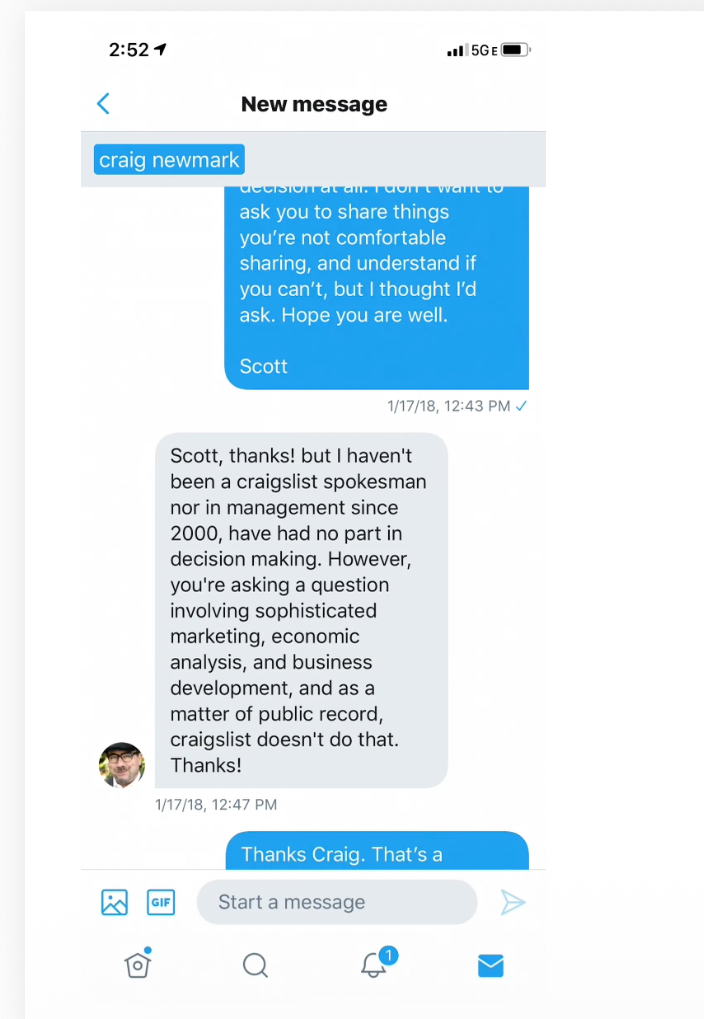
\includegraphics[width=0.62\paperwidth,height=0.94\paperheight,keepaspectratio]{figures/craig_newmark_dm.png}
\end{center}
\end{frame}

\begin{frame}{Checklist step 4: pick your comparison group}
\vspace{0.6em}
\begin{itemize}\setlength\itemsep{0.7em}
  \item Nobody knows the selection rules behind treatment assignment if even Craigslist won't tell anyone.
  \item So I used my best judgment and went with the \highlight{2008--2010} group as my comparison.
  \item My reasoning was simple: at least they got treated eventually.
\end{itemize}
\end{frame}

%% ---------- DRAMATIC SKIP ----------
\begin{frame}
\vfill
\begin{center}
{\Large\color{charcoal} I'm going to skip ahead for the sake of drama.}
\end{center}
\vfill
\end{frame}

%% ---------- STEP 7: PLOT OUTCOMES ACROSS COHORTS ----------
\begin{frame}{Checklist step 7: plot outcomes across cohorts}
\vspace{0.5em}
\begin{itemize}\setlength\itemsep{0.7em}
  \item Make a \highlight{beautiful figure} showing the mean outcomes by cohort.
  \item Remember, we don't care about selection on levels, only selection on \highlight{trends}, and we do see signs of it.
  \item The earlier cohorts have \highlight{flatter trends} than the rest.
  \item Nevertheless, that is what we are doing.
\end{itemize}
\end{frame}

\begin{frame}{Checklist step 7: plot outcomes across cohorts}
\begin{center}
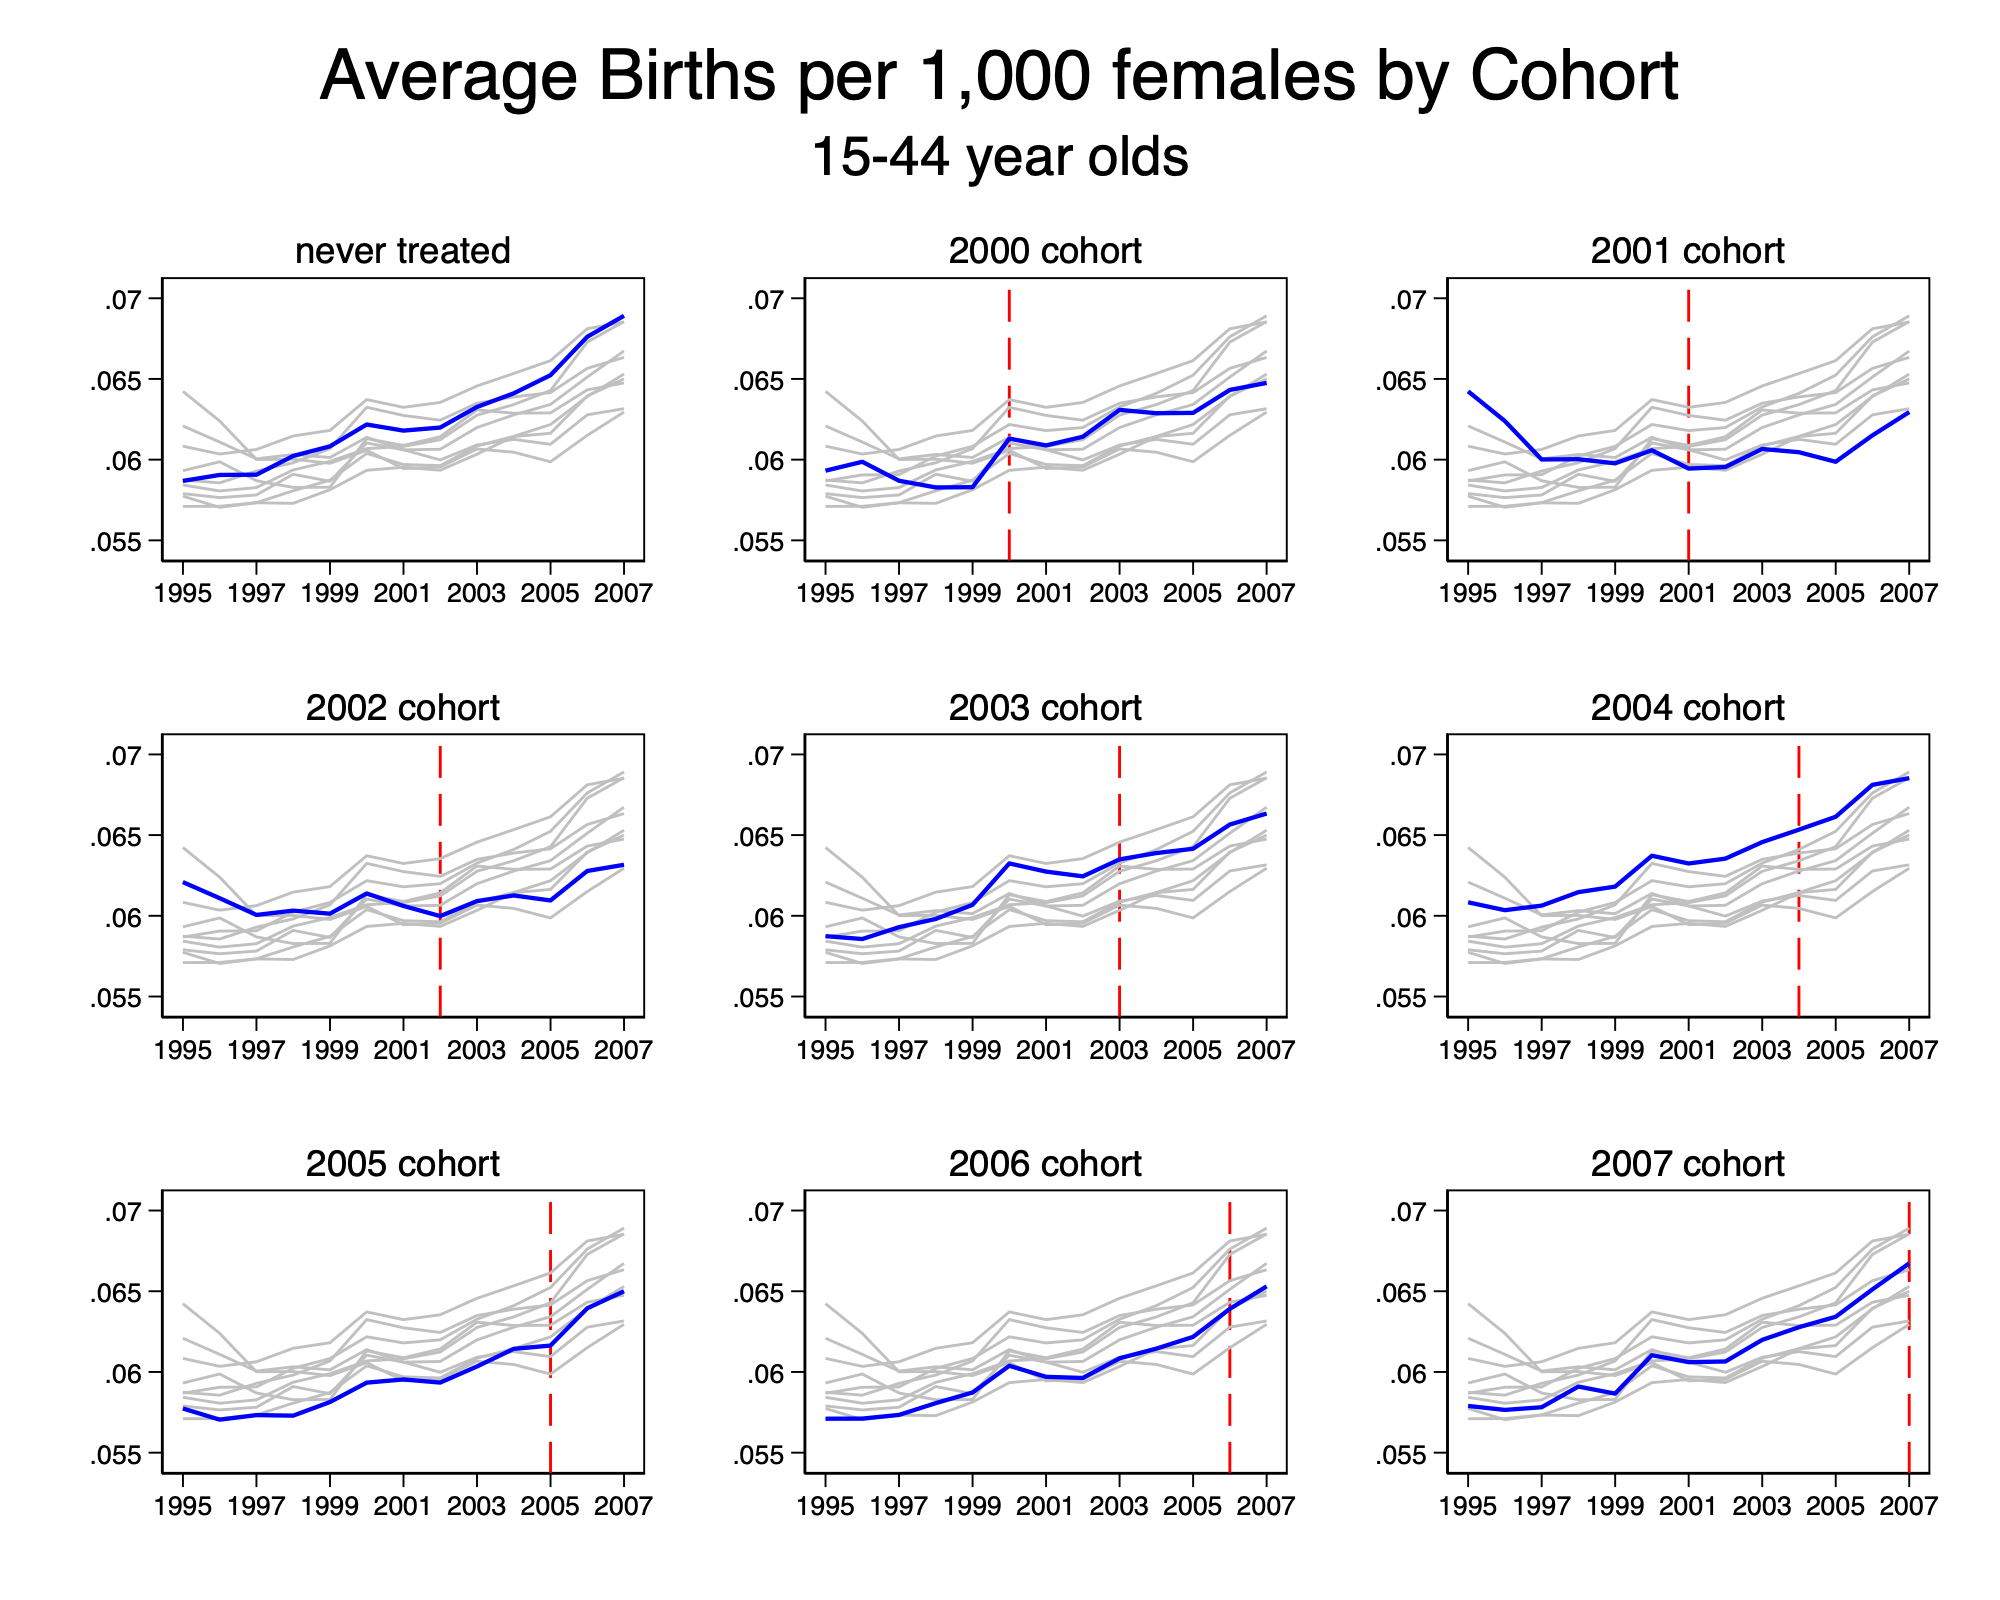
\includegraphics[width=\linewidth,height=0.82\textheight,keepaspectratio]{figures/pretty_outcomes.png}
\end{center}
\end{frame}

%% ---------- STEP 8: ESTIMATOR SELECTION ----------
\begin{frame}{Checklist step 8: estimator selection and assumptions}
\vspace{0.4em}
\begin{itemize}\small\setlength\itemsep{0.45em}
  \item \textbf{Estimator choice:} choose an estimator based on comfort and assumptions.
  \item \textbf{Robust method:} use robust methods like CS, SA, dCDH, or BJS if agnostic to heterogeneous effects.
  \item \textbf{Event study:} estimate simple averages as well as event studies.
  \begin{itemize}\small
    \item Here I used the default syntax in Stata for event studies.
  \end{itemize}
  \item \textbf{Cluster standard errors:} report with clustering at the aggregate level of treatment.
\end{itemize}
\end{frame}

%% ---------- CS ESTIMATOR ----------
\begin{frame}{The Callaway \& Sant'Anna estimator (the IPW version)}
\vspace{1.0em}
\[
\text{ATT}(g,t) = \mathbb{E}\!\left[ \left( \frac{G_g}{\mathbb{E}[G_g]} - \frac{\dfrac{\hat{p}(X)\,C}{1-\hat{p}(X)}}{\mathbb{E}\!\left[\dfrac{\hat{p}(X)\,C}{1-\hat{p}(X)}\right]} \right) \bigl(Y_t - Y_{g-1}\bigr) \right]
\]
\vspace{0.6em}
\begin{itemize}\small\setlength\itemsep{0.45em}
  \item There is an IPW version, an outcome-regression version, and a doubly-robust version, and Sant'Anna recommends \highlight{doubly robust}.
  \item CS uses the never-treated or the not-yet-treated as controls, \highlight{never the already-treated}.
\end{itemize}
\end{frame}

%% ---------- MY CHOICES ----------
\begin{frame}{My choices}
\vspace{1.0em}
\begin{itemize}\setlength\itemsep{1.0em}
  \item I will use \highlight{CS} because it is simple (four averages and three subtractions) and popular.
  \item I will not use covariates.
  \item I will make an event study.
\end{itemize}
\end{frame}

\begin{frame}{Short-gaps, no controls}
\begin{center}
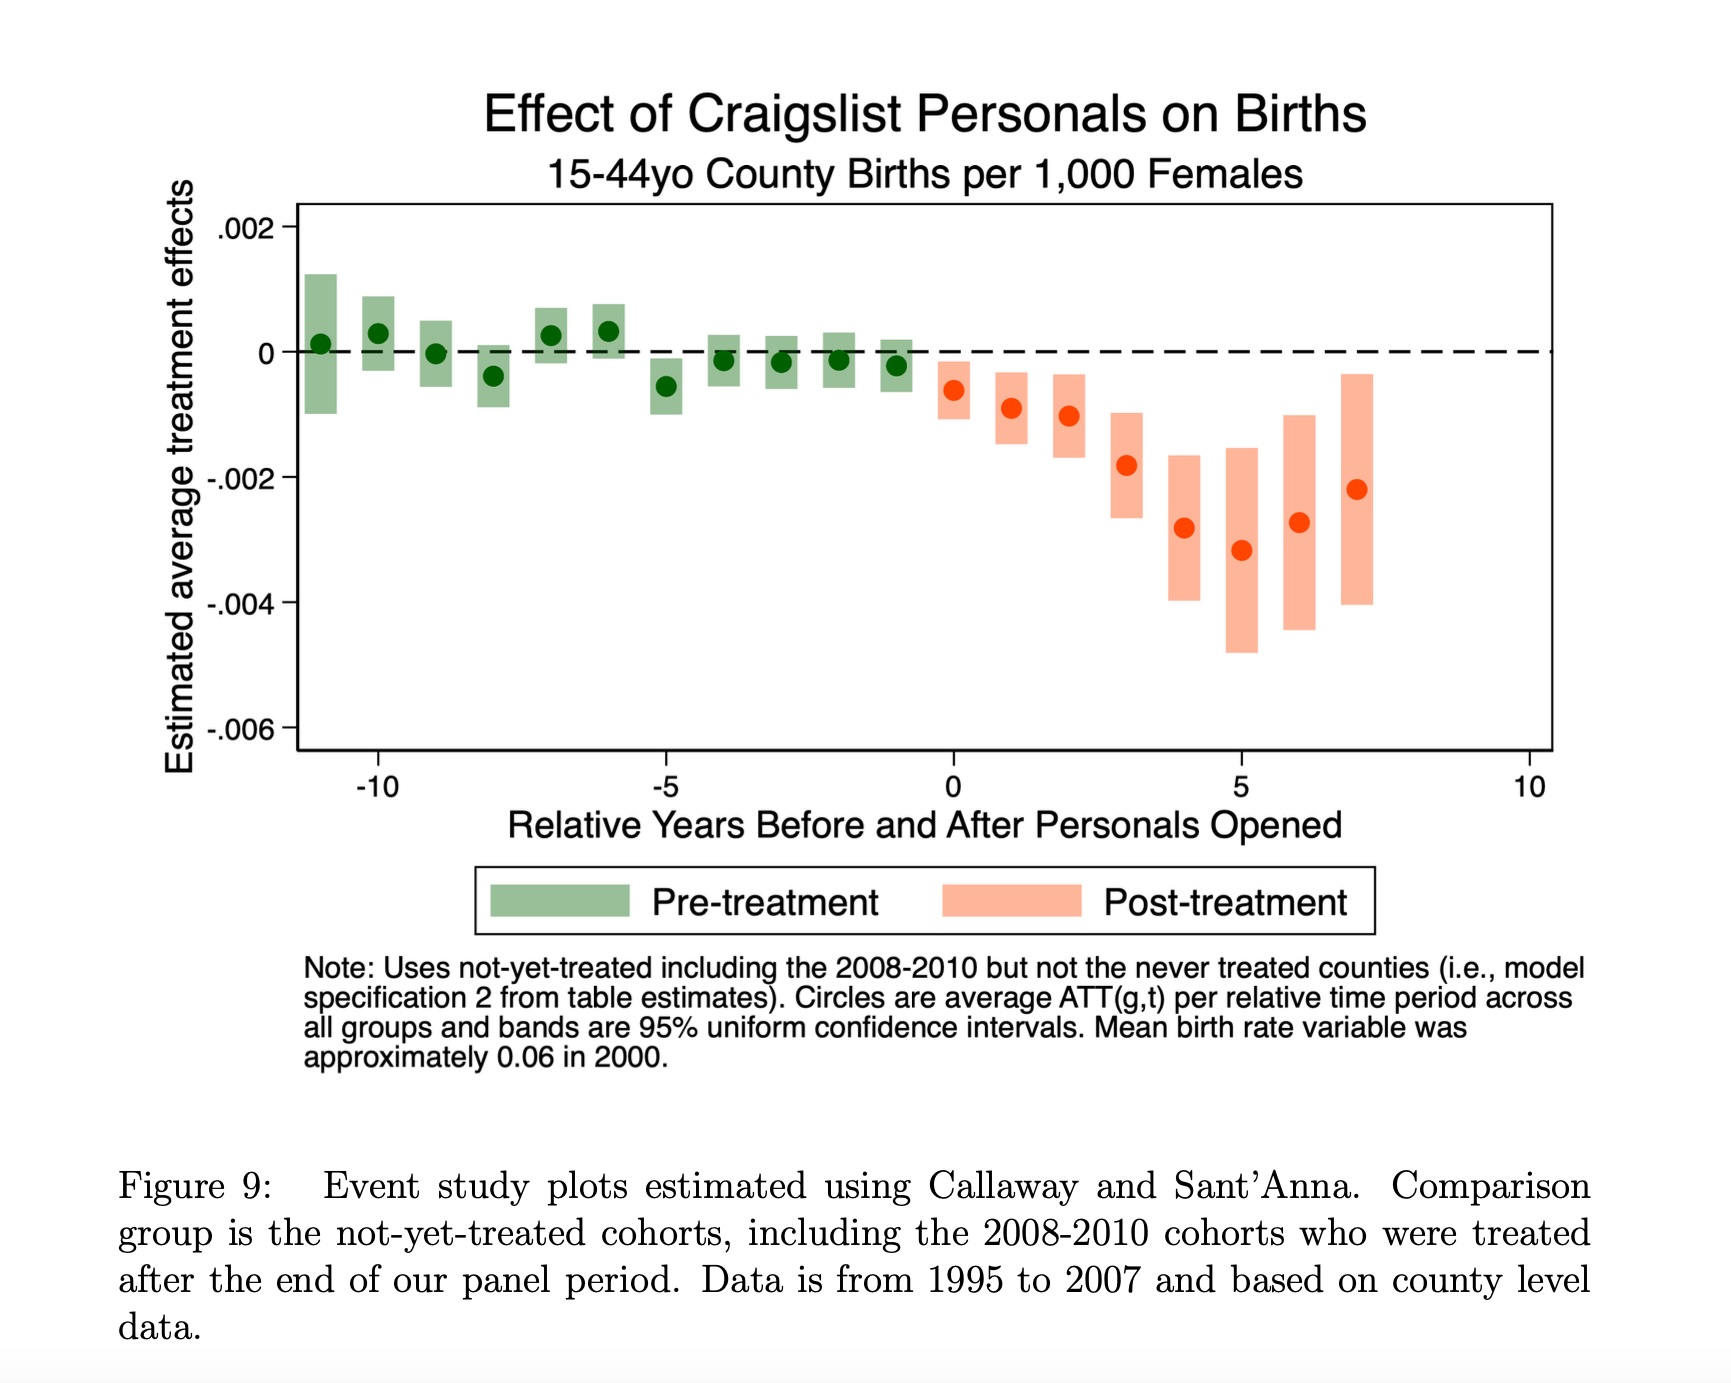
\includegraphics[width=\linewidth,height=0.82\textheight,keepaspectratio]{figures/es_births_shortgapNC.jpg}
\end{center}
\end{frame}

%% ---------- DOUBT ENSUED ----------
\begin{frame}[shrink=5]{Doubt ensued}
\vspace{0.3em}
\begin{itemize}\small\setlength\itemsep{0.5em}
  \item The event study plots persuaded us that unconditional parallel trends was reasonable.
  \item But then I learned about a ``software default'' in both R and Stata.
  \item If you do not specify \texttt{long2} in \texttt{csdid}, or \texttt{base\_period="universal"} in R, the default is short gaps.
  \item I had always taught long differences, and it never occurred to me that this wasn't doing that (double-check the 2$\times$2).
  \item But my event study plots looked so good, and I already had a narrative about ``permanent dating''!
\end{itemize}
\end{frame}

%% ---------- TRENDS OR NO TRENDS (side by side) ----------
\begin{frame}{Trends or no trends?!}
\vspace{0.3em}
\begin{columns}[T]
\begin{column}{0.5\textwidth}
\centering
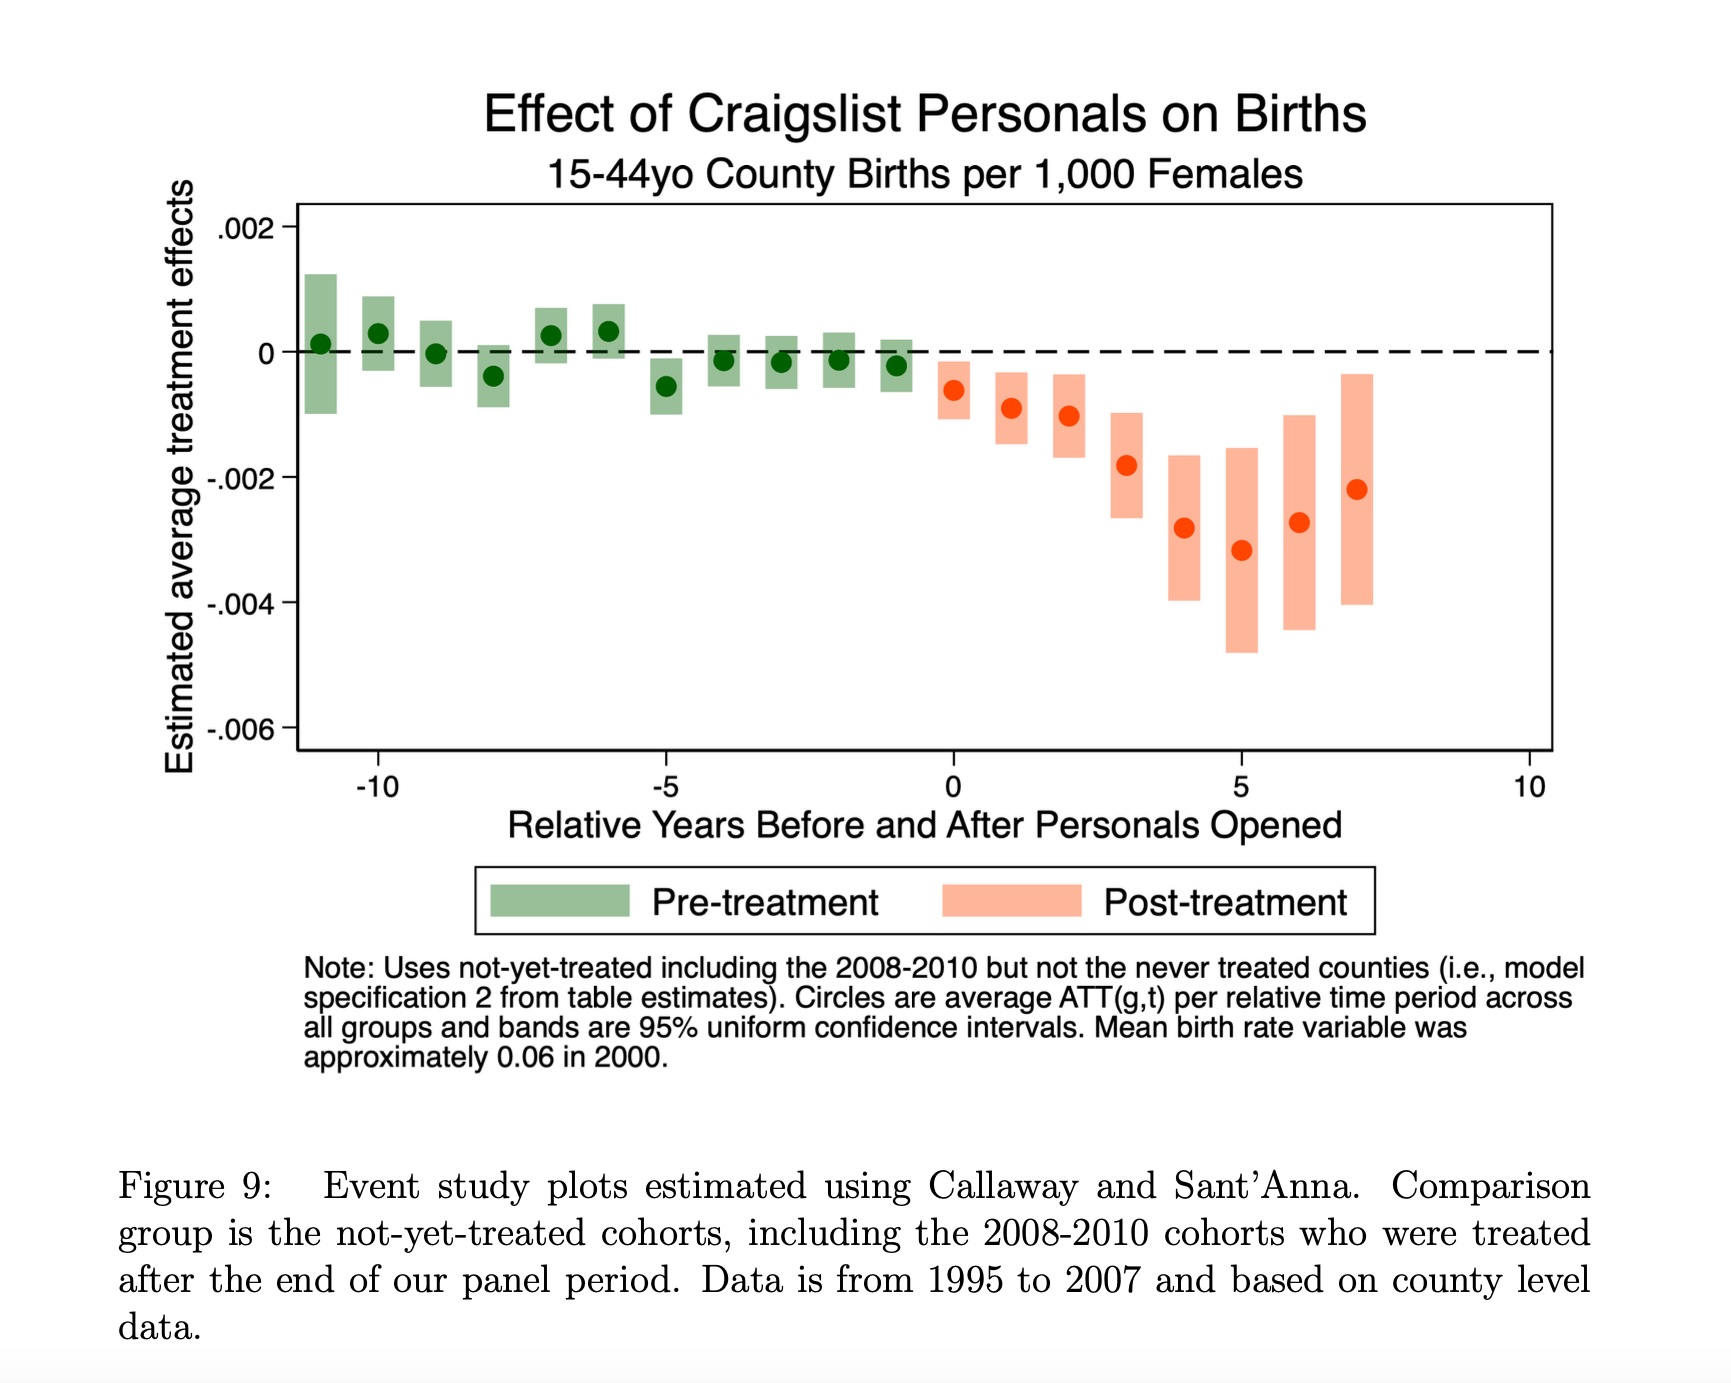
\includegraphics[width=\linewidth,height=0.72\textheight,keepaspectratio]{figures/es_births_shortgapNC.jpg}\\[0.3em]
{\itshape\small Short gap}
\end{column}
\begin{column}{0.5\textwidth}
\centering
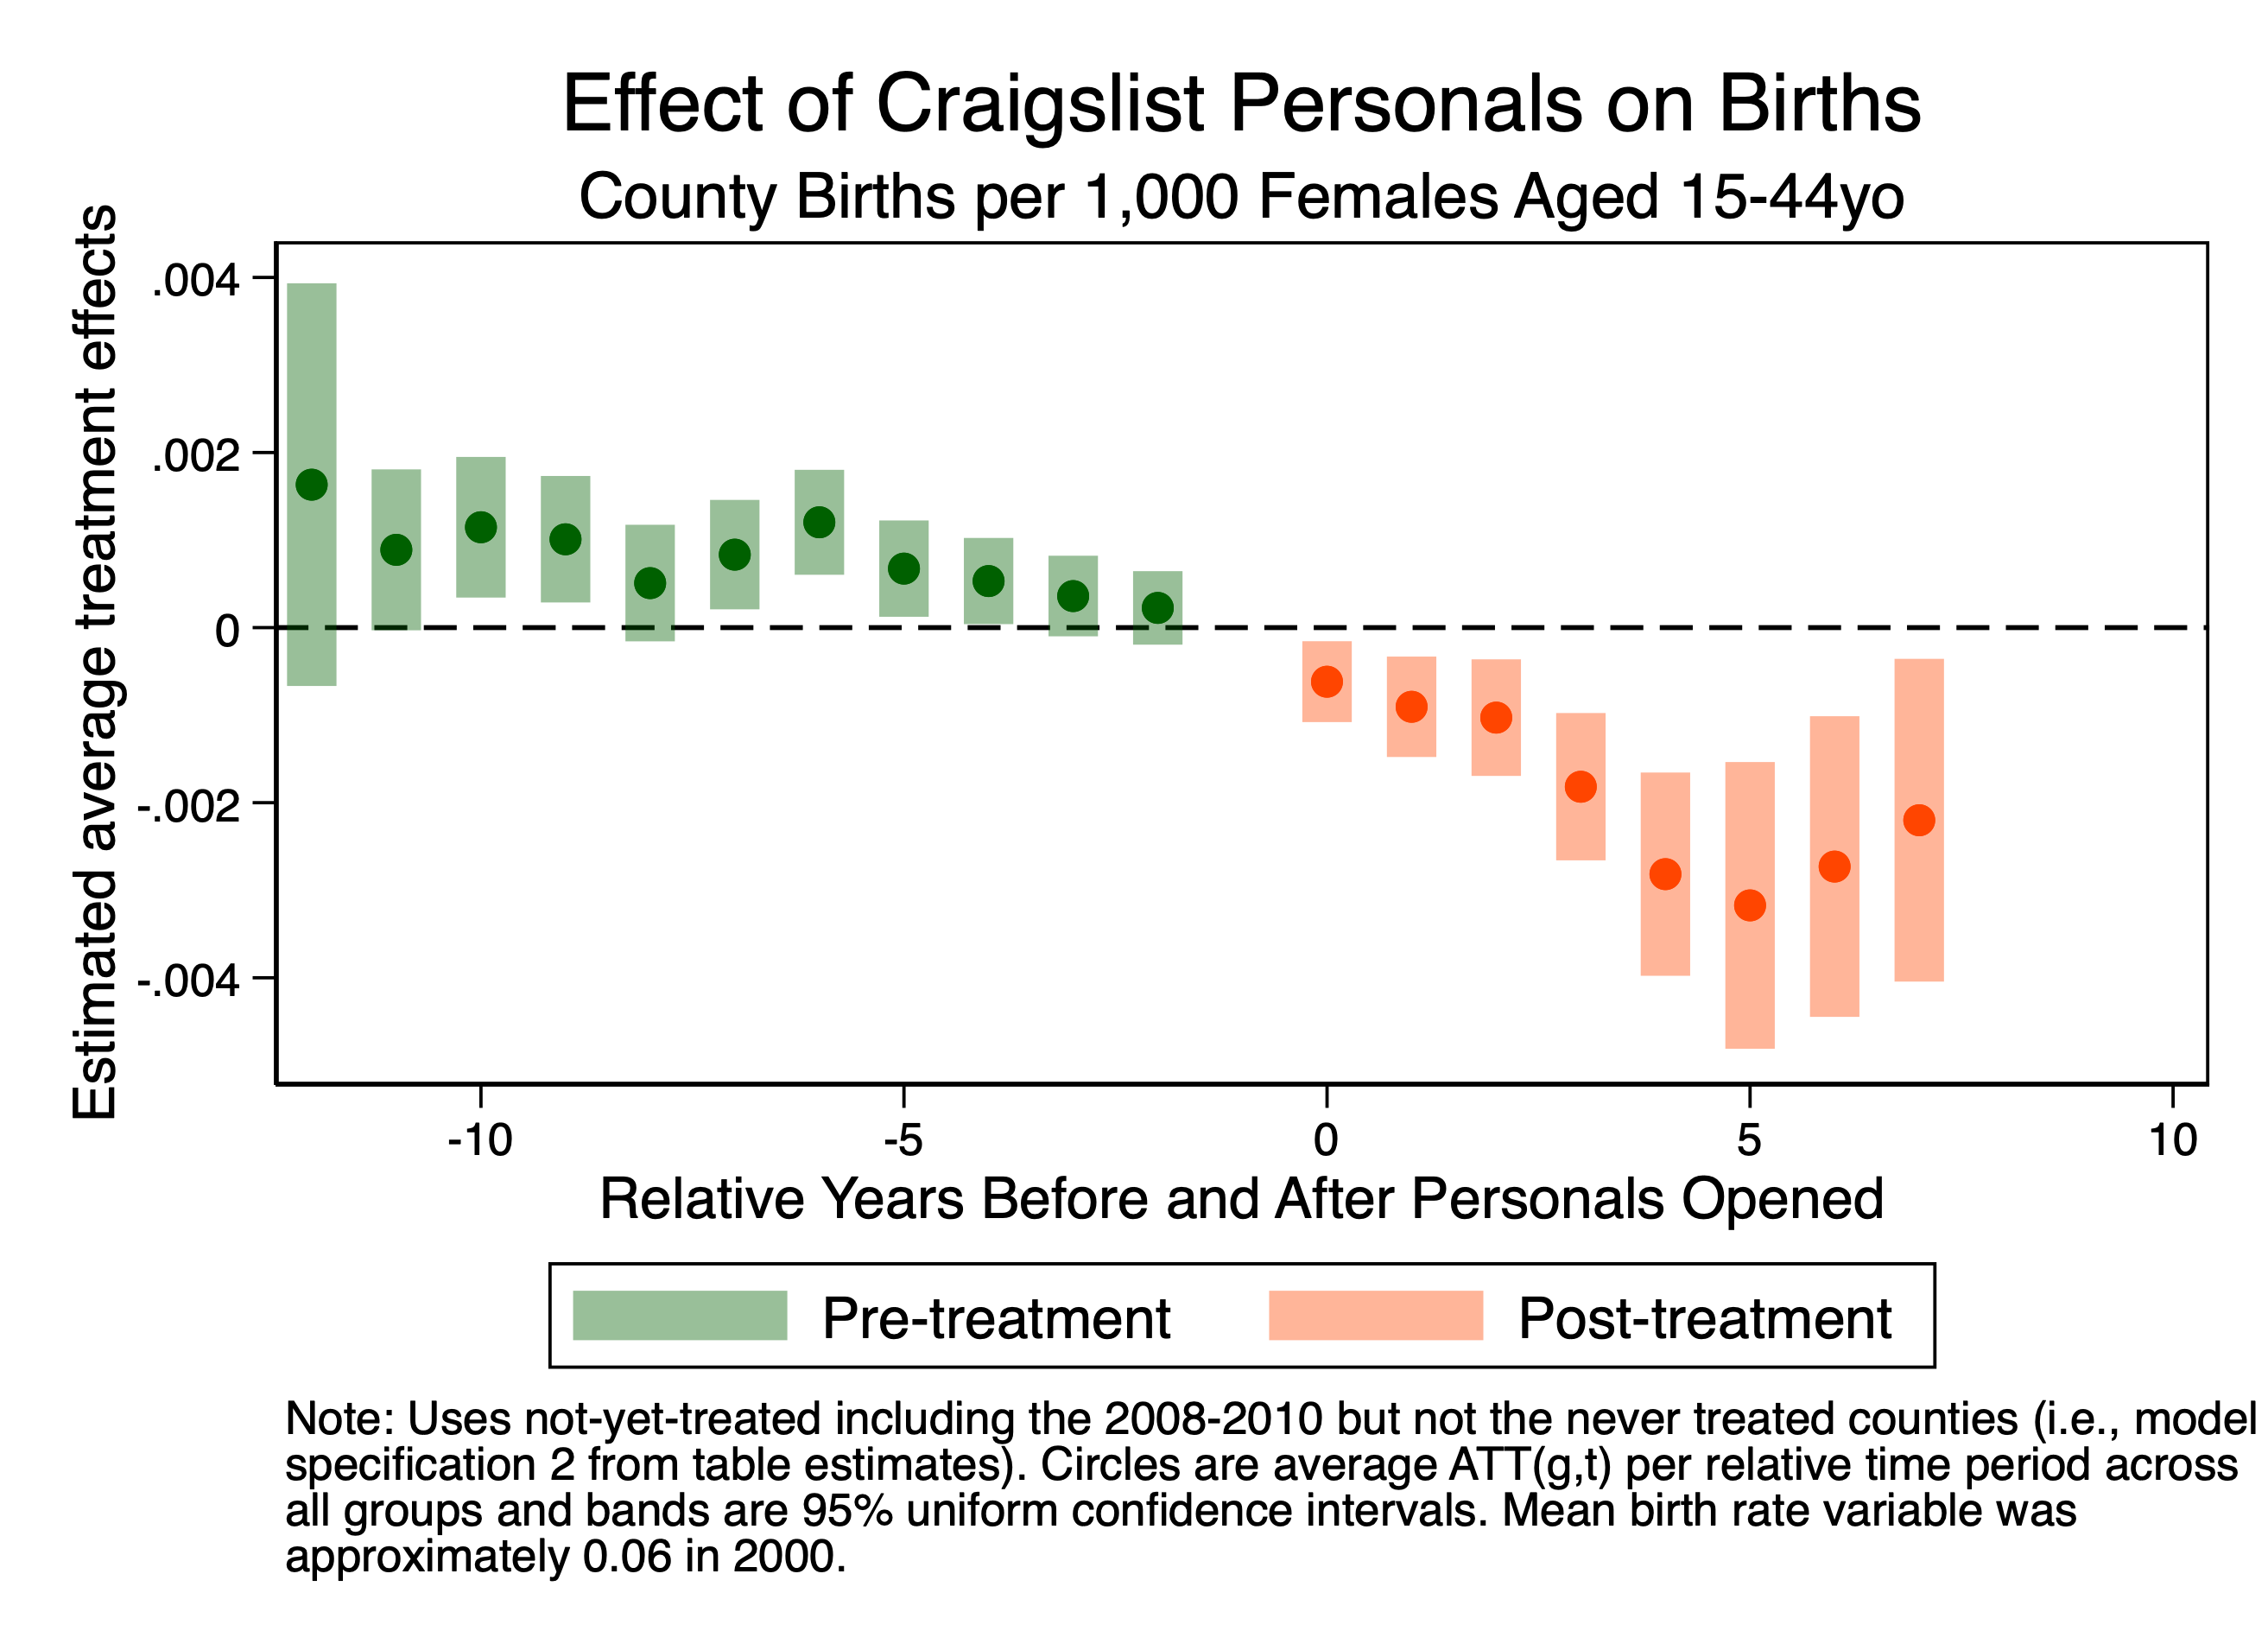
\includegraphics[width=\linewidth,height=0.72\textheight,keepaspectratio]{figures/es_births2.png}\\[0.3em]
{\itshape\small Long difference}
\end{column}
\end{columns}
\end{frame}

%% ---------- SCRUTINIZING ----------
\begin{frame}[shrink=5]{Scrutinizing that event study}
\vspace{0.3em}
\begin{itemize}\small\setlength\itemsep{0.5em}
  \item I was so excited when I saw those flat pre-trends, until I learned that the default syntax in Stata's \texttt{csdid} calculated short gaps.
  \item We had a whole story that online dating caused ``permanent dating,'' until I realized that, lol.
  \item But that made us start wondering whether unconditional parallel trends was plausible.
  \item We started to piece together what our different units were, that is, ``counties'' who were treated versus ``counties'' who weren't.
  \item Why would some counties get a Craigslist but not others?
\end{itemize}
\end{frame}

%% ---------- WHO GOT A CRAIGSLIST ----------
\begin{frame}{Who got a Craigslist and who didn't?}
\vspace{0.6em}
\begin{itemize}\setlength\itemsep{0.8em}
  \item Craigslist is organized by city, like \texttt{houston.craigslist.org} for Houston, Texas.
  \item I grew up in Brookhaven, Mississippi, a town of 11,000, and \texttt{brookhaven.craigslist.org} is not there.
  \item Craigslist targeted cities, but most US counties are rural.
\end{itemize}
\end{frame}

%% ---------- IS UNCONDITIONAL PT PLAUSIBLE? ----------
\begin{frame}[shrink=8]{Is unconditional parallel trends plausible?}
\vspace{0.2em}
\begin{itemize}\small\setlength\itemsep{0.45em}
  \item My coauthors are demographers with a 20-year research agenda in maternal health and children.
  \item We are all labor economists, familiar with ``sorting'' into rural versus cities and how population characteristics differ:
  \begin{itemize}\small\setlength\itemsep{0.25em}
    \item Cities have more college-educated women, delayed childbearing, lower marriage rates, different racial composition, and more access to female healthcare.
    \item Rural towns have less-educated women, earlier age at first birth, higher marriage rates, more homogeneity, and worse healthcare access.
  \end{itemize}
  \item If Craigslist counties are more urban, then treatment and control are imbalanced on covariates that cause trends in $Y^0$.
  \item So we looked at mean female population and urban measures by timing cohort to see how bad the covariate imbalance was.
\end{itemize}
\end{frame}

\begin{frame}{Long differences without and with RUCC control (!)}
\begin{center}
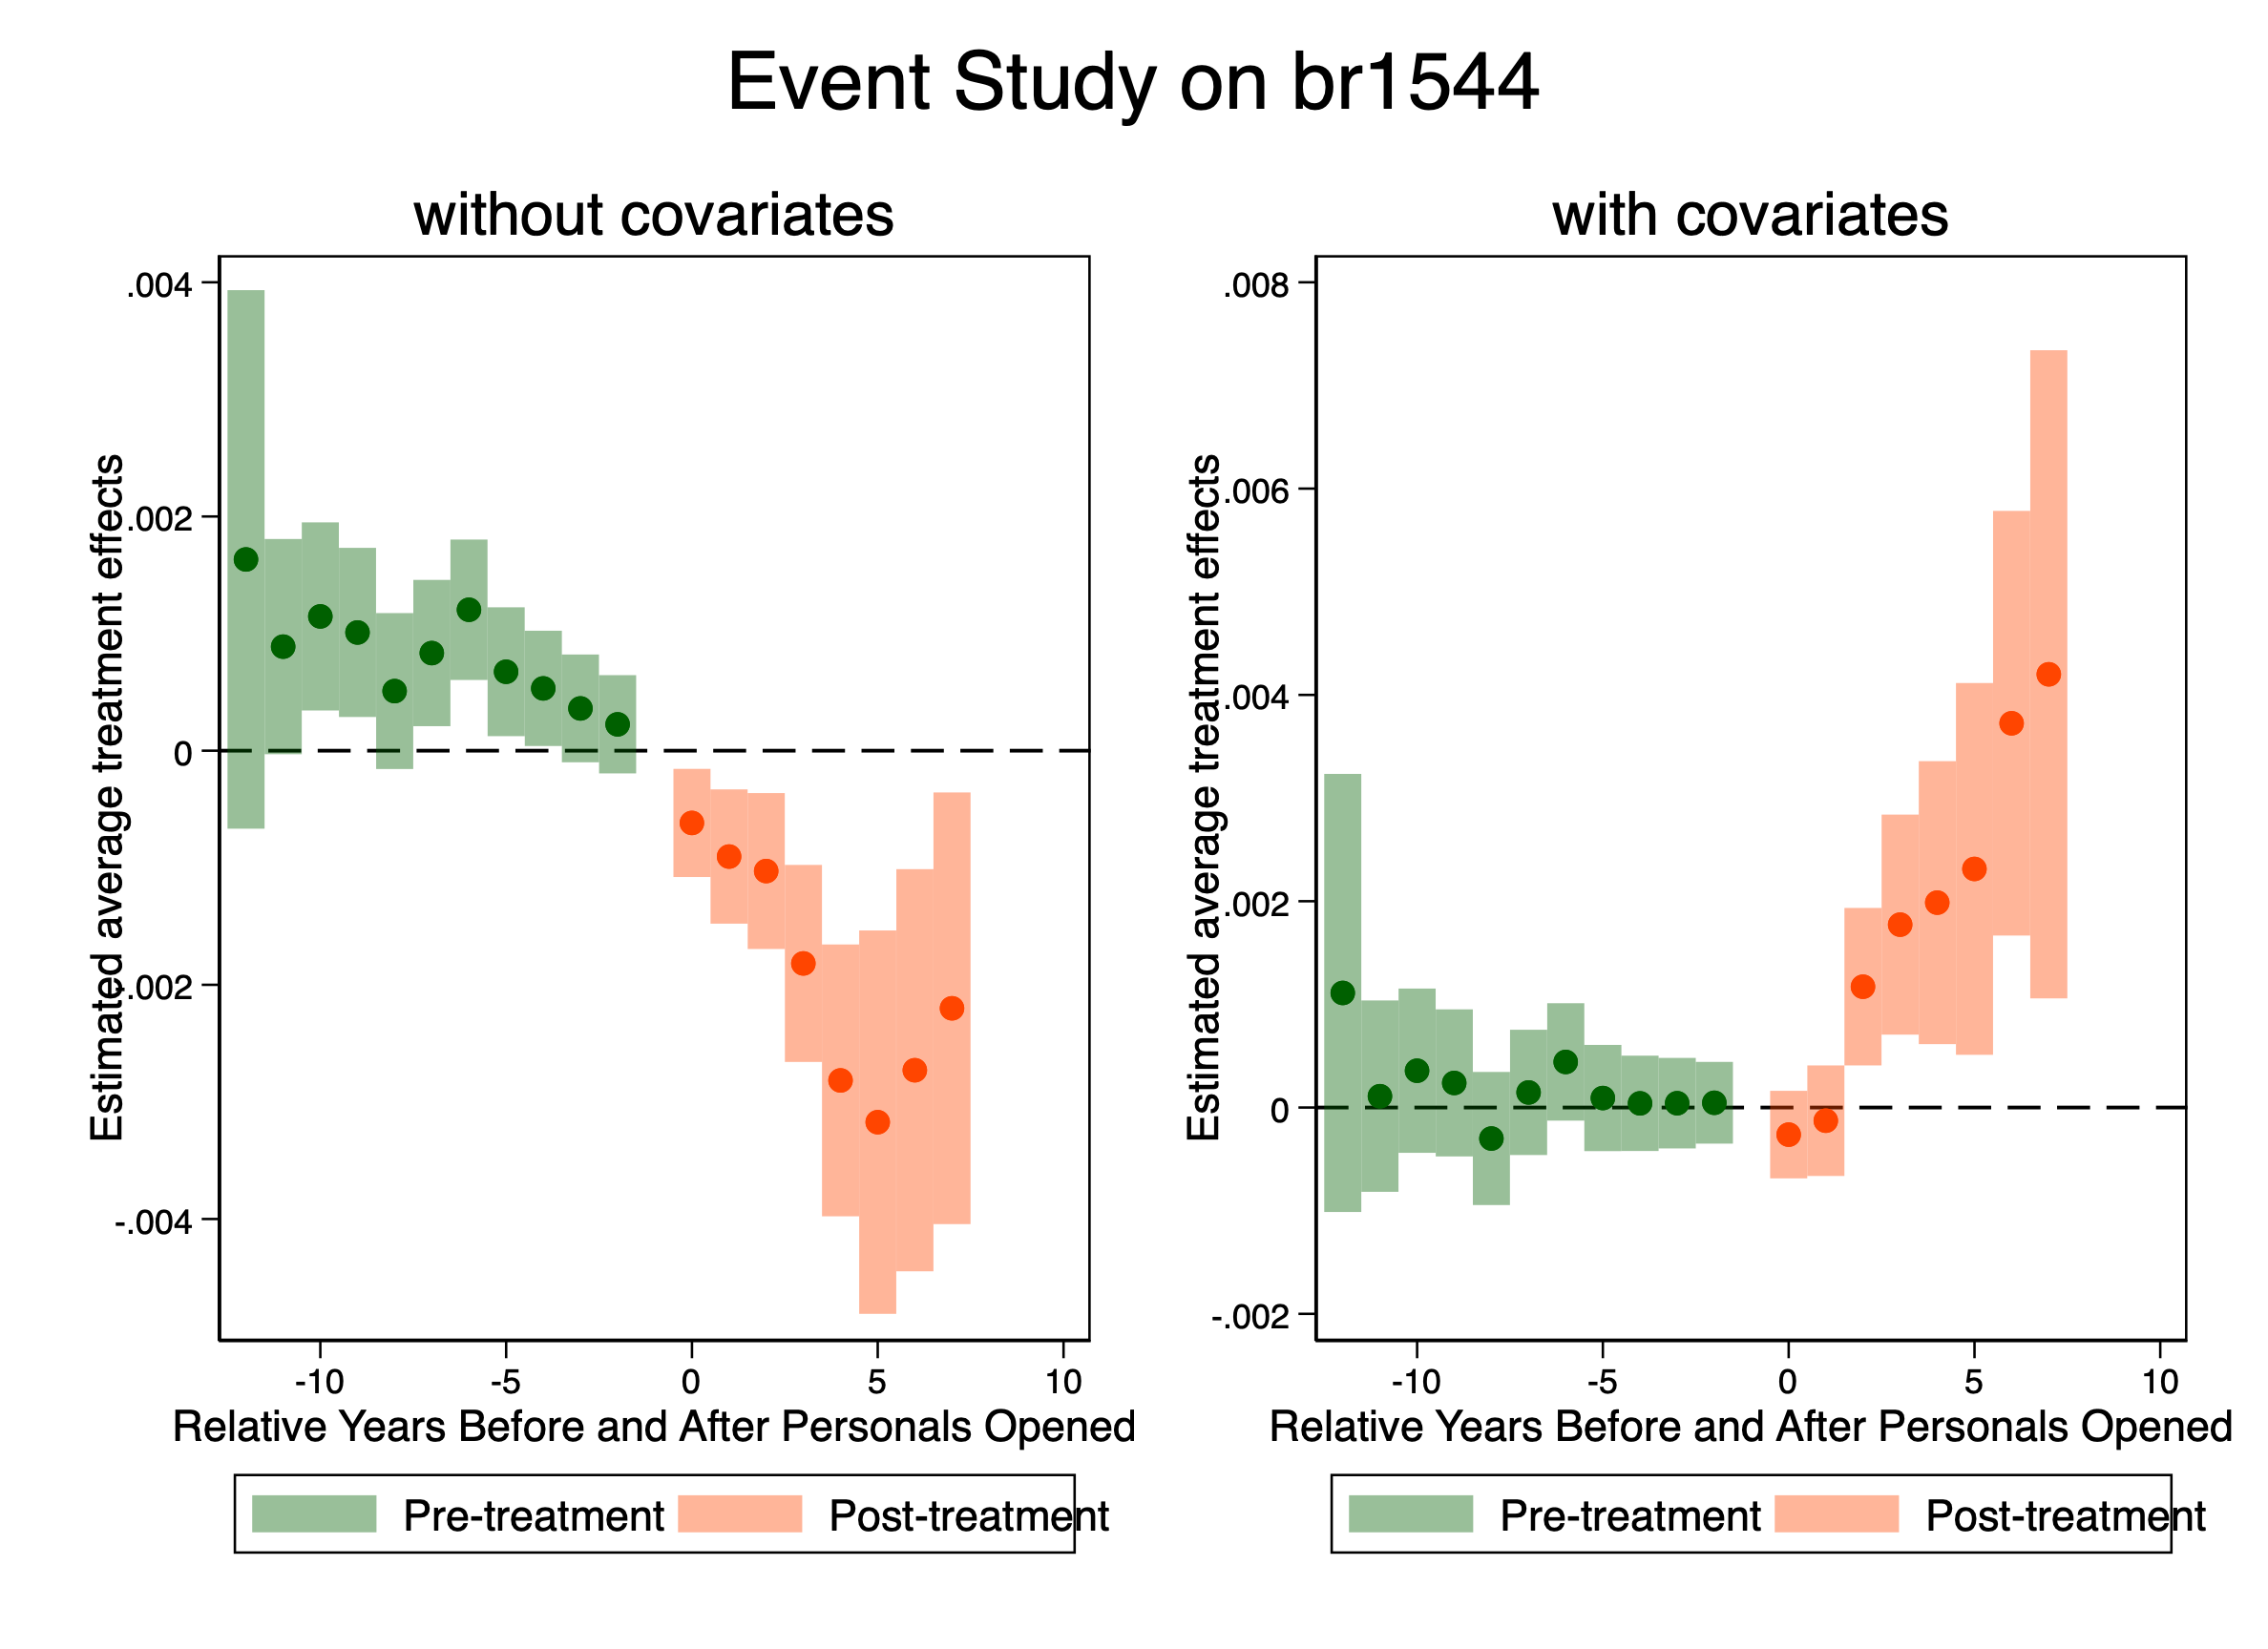
\includegraphics[width=\linewidth,height=0.82\textheight,keepaspectratio]{figures/es_br1544_combined.png}
\end{center}
\end{frame}

\begin{frame}{Running it within each RUCC code}
\begin{center}
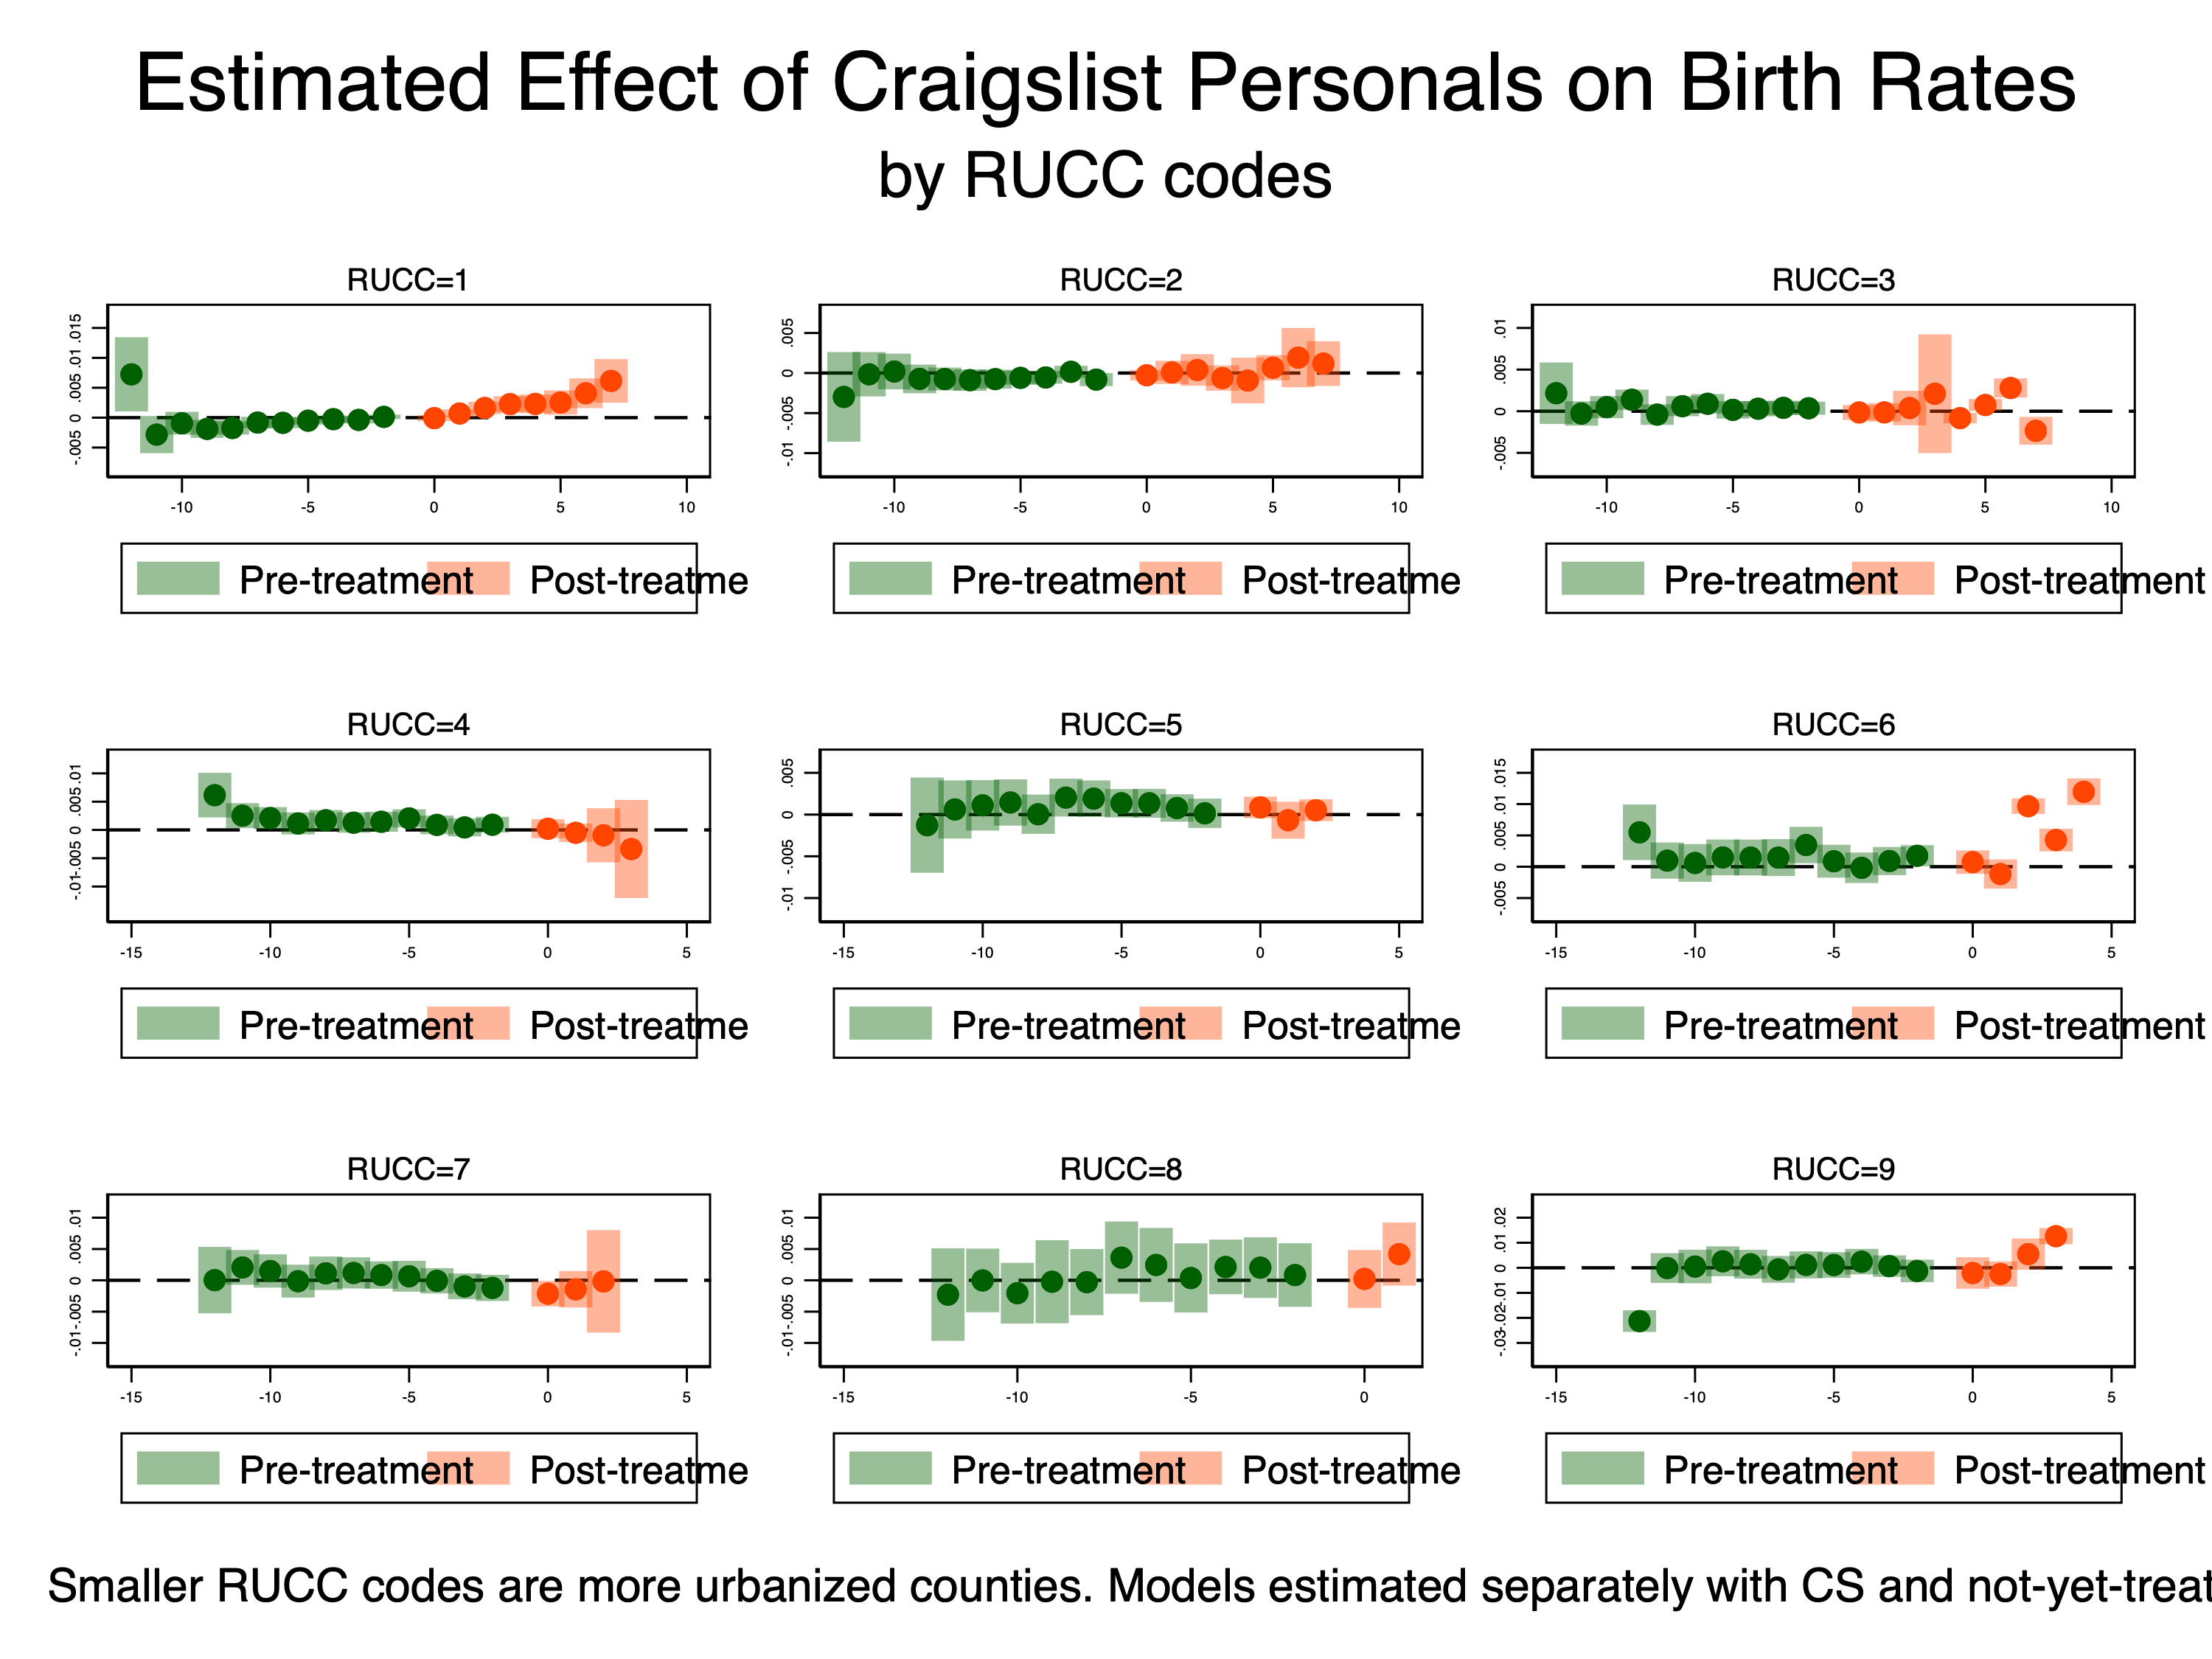
\includegraphics[width=\linewidth,height=0.82\textheight,keepaspectratio]{figures/es_br1544_RUCCcombined.png}
\end{center}
\end{frame}

%% ---------- STEP 3 ----------
\begin{frame}{Checklist step 3: validity of unconditional parallel trends}
\vspace{0.5em}
\begin{enumerate}
\item[3.] Validity of the unconditional parallel trends assumption
\end{enumerate}
\vspace{0.4em}
\begin{itemize}\small\setlength\itemsep{0.45em}
  \item \textbf{Covariate selection:} choose covariates predictive of the missing potential outcome based on common sense, literature, and expertise.
  \item \textbf{Split-sample validation:} use untreated outcomes with methods like Lasso to identify covariates if unsure.
  \item \textbf{Balance check:} check covariate balance using normalized differences.
  \item \textbf{Adjust imbalanced covariates:} adjust if covariates are predictive of $[Y^0 \mid D{=}1,\text{Post}]$.
\end{itemize}
\end{frame}

\begin{frame}{Rural vs.\ urban counties}
\vspace{0.4em}
\begin{itemize}\setlength\itemsep{0.5em}
  \item We have a 9-digit ordinal score measuring how urbanized a county is, called \highlight{RUCC}.
  \item Counties that never got a Craigslist were \highlight{more rural}.
  \item We had originally wanted to use the 2008--2010 and other not-yet-treated counties as comparisons.
  \item I'll \highlight{plot} rather than report the normalized difference, for illustrative purposes.
\end{itemize}
\end{frame}

\begin{frame}{Plotting covariate imbalance}
\begin{center}
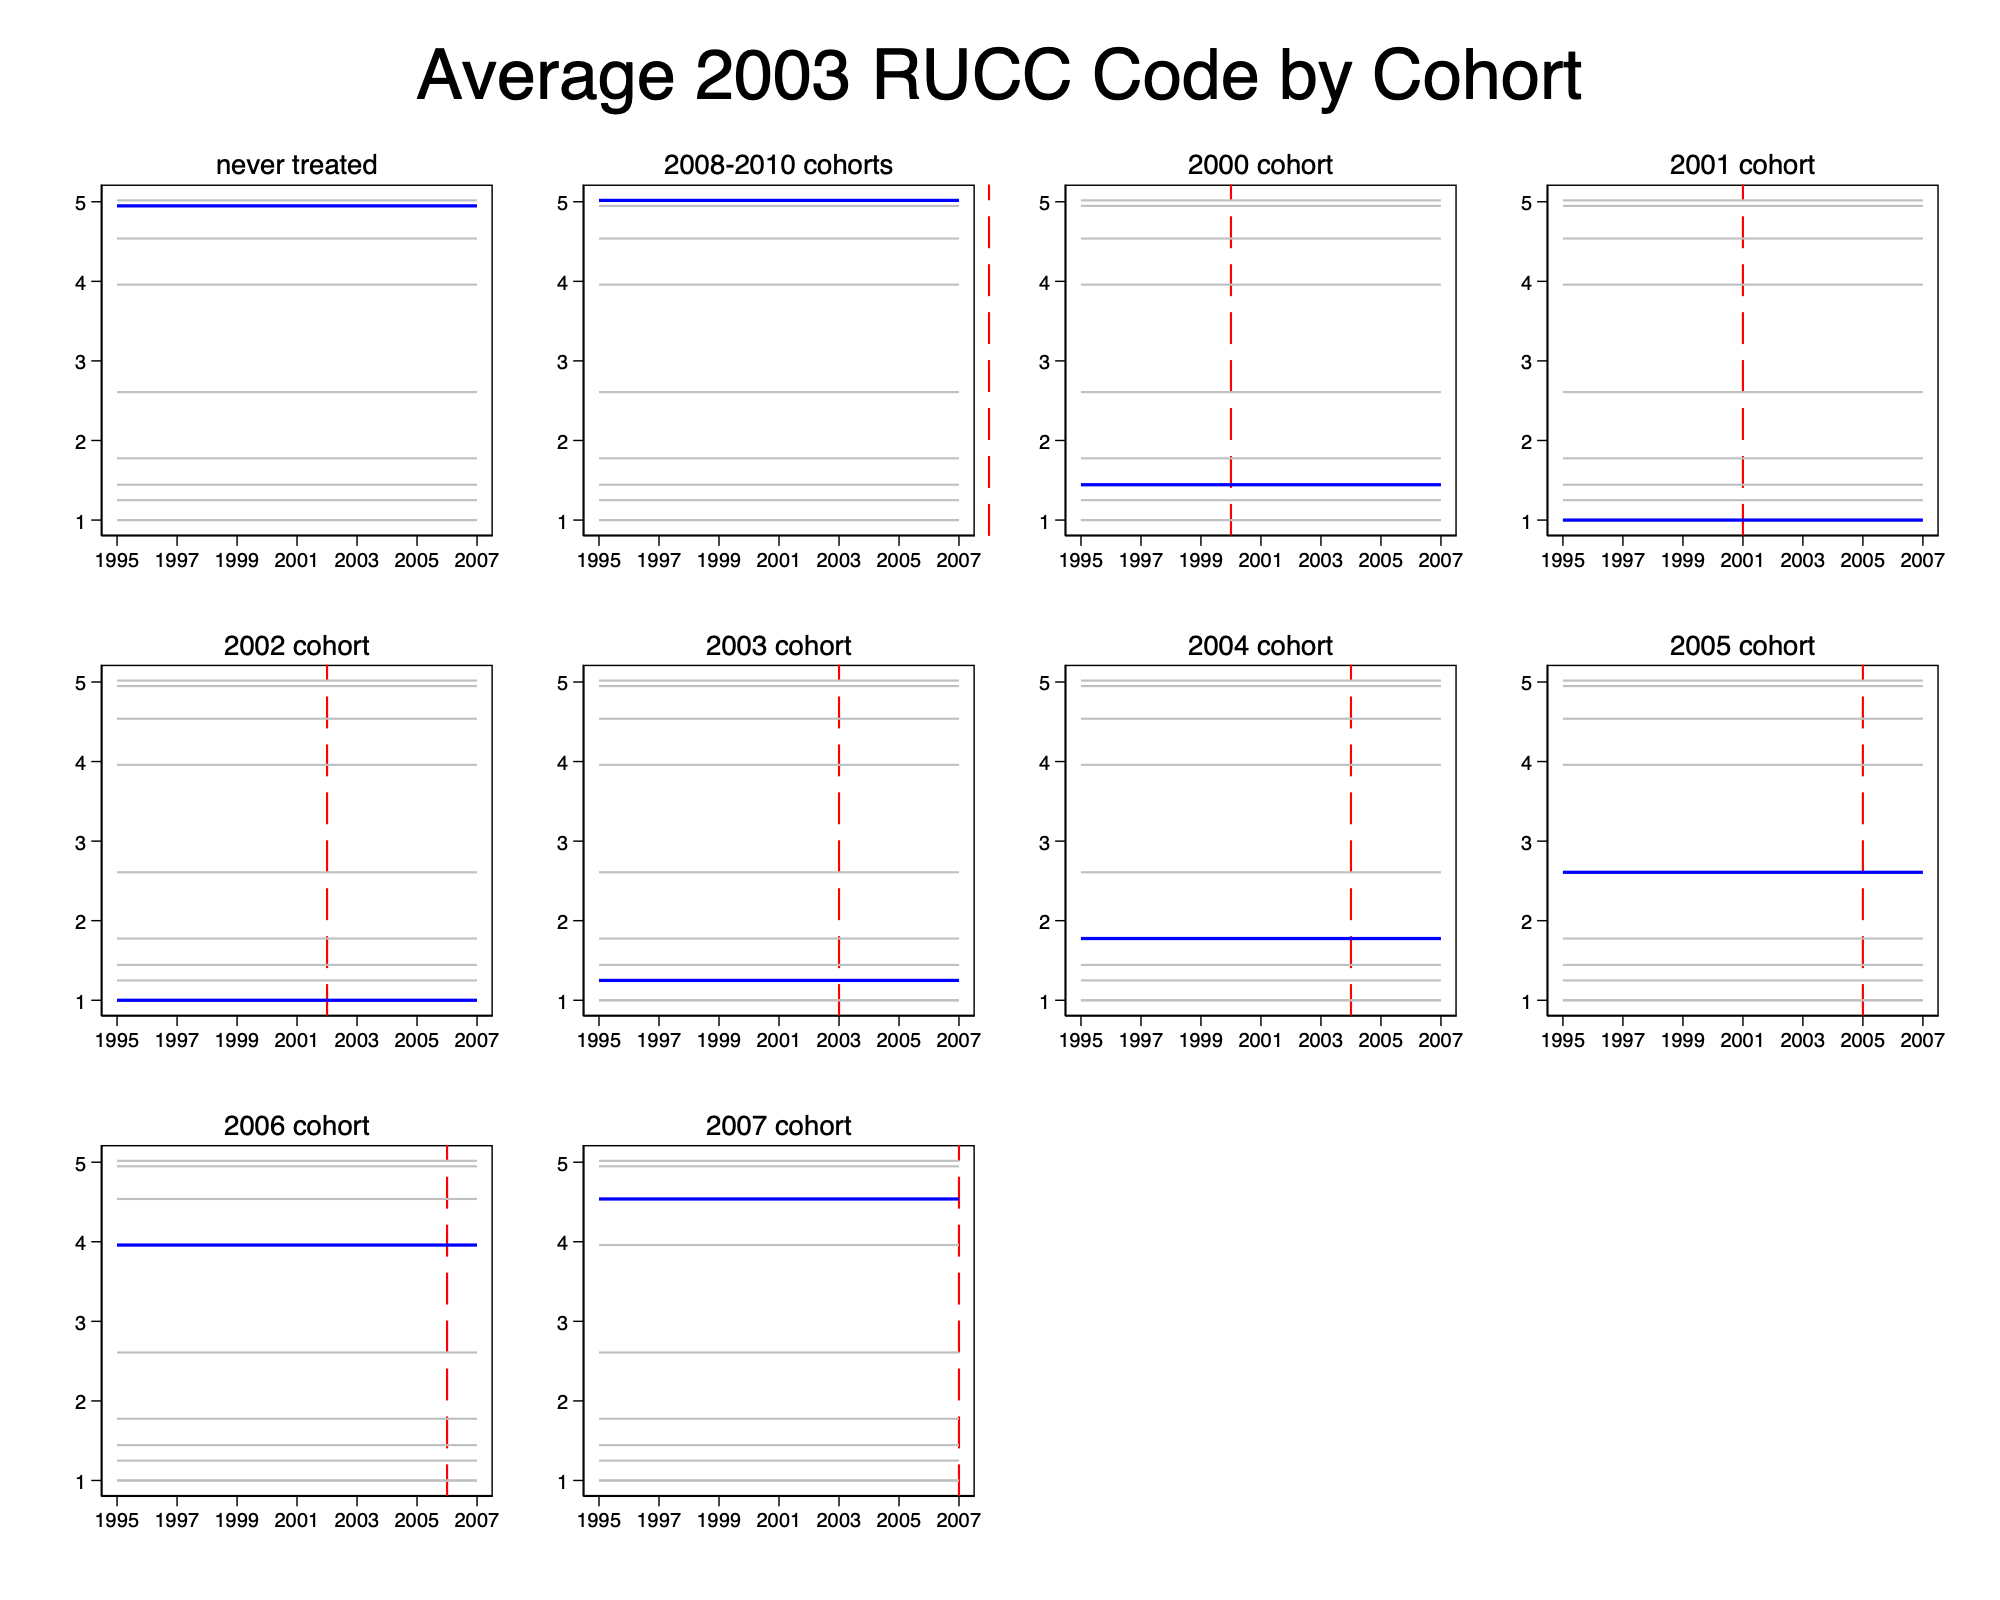
\includegraphics[width=\linewidth,height=0.82\textheight,keepaspectratio]{figures/pretty_RUCC.png}
\end{center}
\end{frame}

\begin{frame}{Comment}
\vspace{0.5em}
\begin{itemize}\setlength\itemsep{0.6em}
  \item Urban counties differ in race, age, sex ratios, education shares, and income, all \highlight{highly predictive} of untreated birth-rate trends.
  \item And even the 2008--2010 counties, despite our hope, are very rural, just as rural, even.
  \item So we will run it \highlight{both ways}: without controls, and then with a single covariate (RUCC).
\end{itemize}
\end{frame}

%% ---------- STEP 4 ----------
\begin{frame}{Checklist step 4: check overlap}
\vspace{0.6em}
\begin{enumerate}
\item[4.] Check overlap
\end{enumerate}
\vspace{0.4em}
\begin{itemize}\small\setlength\itemsep{0.45em}
  \item \textbf{Overlap check:} ensure sufficient overlap in propensity scores.
  \item \textbf{Adjustment for lack of overlap:} if lacking, consider a regression adjustment like BJS.
  \item We have overlap since the RUCC code has only 9 values, so I'll skip it here, but you'll want to check using a \highlight{propensity score} if you have continuous or several covariates.
\end{itemize}
\vspace{0.4em}
\emphbox{\textbf{Watch for perfect separation.} With a propensity-score model, a covariate that perfectly predicts treatment forces $\hat p(X) \to 0$ or $1$, weights blow up, and the estimator is undefined. Few discrete covariate values (like RUCC) keep you safe; rich or continuous covariates do not.}
\end{frame}

%% ---------- STEP 6 ----------
\begin{frame}{Checklist step 6: sensitivity analysis for PT violations}
\vspace{0.6em}
\begin{enumerate}
\item[6.] Sensitivity analysis for parallel-trends violations
\end{enumerate}
\vspace{0.4em}
\begin{itemize}
  \item \textbf{Consider sensitivity analysis:} use tools like \texttt{honestdid} for PT violations.
\end{itemize}
\end{frame}

%% ---------- STEP 7 ----------
\begin{frame}{Checklist step 7: throw in the towel}
\vspace{0.4em}
\begin{enumerate}
\item[7.] Throw in the towel
\end{enumerate}
\vspace{0.3em}
\begin{itemize}\small\setlength\itemsep{0.4em}
  \item You may have to concede that, for any number of reasons, parallel trends with or without covariates is implausible, it happens.
  \item Consider some alternatives:
  \begin{itemize}\small
    \item \textbf{Panel method:} if imbalance or PT fails, consider matrix completion or nuclear-norm regularization.
    \item \textbf{Cross-section:} cross-sectional unconfoundedness may also be appropriate.
  \end{itemize}
  \item Don't force it, diff-in-diff doesn't make estimates causal; \highlight{parallel trends makes diff-in-diff causal}.
\end{itemize}
\end{frame}

%% ============================================================
%% CONCLUDING REMARKS
%% ============================================================
\remixsection{Concluding Remarks}

\begin{frame}{Concluding remarks on DiD}
\vspace{0.3em}
\begin{itemize}\small\setlength\itemsep{0.45em}
  \item You're probably going to write a paper using DiD at least once in your life, probably more.
  \item Even if you don't, you'll read many DiD papers, referee them, or advise students using them.
  \item It's in your interest to make the fixed-cost investment in the new econometrics of DiD, because the old methods are mostly harmful.
  \item Good news: we are at the conclusion of this wave of papers, software is now widely available, and solutions share common features, static and dynamic presentations aren't all that different.
  \item Lots of surveys exist (Roth et al.\ 2023; our new JEL), and you'll have the slides and recordings.
\end{itemize}
\end{frame}

\begin{frame}{Concluding remarks: covariates}
\vspace{0.4em}
\begin{itemize}\setlength\itemsep{0.55em}
  \item Stronger assumptions are needed to include covariates, and the bias can be large.
  \item You need the \highlight{correct} covariates, I suggested sample splitting for selection and Lasso to identify covariates that affect \textbf{untreated potential outcomes}.
  \item Don't control for covariates that could be affected by the outcome.
\end{itemize}
\end{frame}

\begin{frame}{Concluding remarks: differential timing}
\vspace{0.3em}
\begin{itemize}\small\setlength\itemsep{0.45em}
  \item The main problem in differential timing is heterogeneity and the use of already-treated units as controls.
  \item With differential timing and no a priori theory, you \emph{should} avoid the canonical TWFE specification.
  \item Under heterogeneity, canonical TWFE is biased, signs can flip, weights can be negative.
  \item Robust DiD methods place no restrictions on treatment-effect heterogeneity, but they can't solve everything.
  \item When you lose parallel trends, you're probably heading toward needing a new design.
\end{itemize}
\end{frame}

\begin{frame}{Concluding remarks: design discipline}
\vspace{0.5em}
\begin{itemize}\setlength\itemsep{0.6em}
  \item Devote time to \highlight{designing} your diff-in-diff, it keeps you honest and surfaces problems before you've peeked at the outcomes.
  \item It's much harder, psychologically, to pull back once you're invested in a story, so don't go to the outcomes until you've pre-registered your study to some degree, even if not formally.
\end{itemize}
\end{frame}

\begin{frame}[plain]
\begin{tikzpicture}[remember picture,overlay]
\fill[cream] (current page.south west) rectangle (current page.north east);
\node[anchor=center, text width=0.84\paperwidth, align=center, text=charcoal]
  at (current page.center) {%
  \fontsize{18pt}{26pt}\selectfont
  Diff-in-diff doesn't make estimates causal.\\[0.6em]
  {\color{accent}\bfseries Parallel trends makes diff-in-diff causal.}
};
\draw[accent, line width=1pt]
  ([yshift=1.4cm,xshift=0.25\paperwidth]current page.south west)
  -- ([yshift=1.4cm,xshift=-0.25\paperwidth]current page.south east);
\end{tikzpicture}
\end{frame}

\end{document}
